\documentclass[a4paper]{article}

\def\npart {III}
\def\nterm {Michaelmas}
\def\nyear {2016}
\def\nlecturer {J. A. Ross}
\def\ncourse {Differential Geometry}
\def\nlectures {MWF.11}

% Imports
\ifx \nextra \undefined
  \usepackage[pdftex,
    hidelinks,
    pdfauthor={Dexter Chua},
    pdfsubject={Cambridge Maths Notes: Part \npart\ - \ncourse},
    pdftitle={Part \npart\ - \ncourse},
  pdfkeywords={Cambridge Mathematics Maths Math \npart\ \nterm\ \nyear\ \ncourse}]{hyperref}
  \title{Part \npart\ - \ncourse}
\else
  \usepackage[pdftex,
    hidelinks,
    pdfauthor={Dexter Chua},
    pdfsubject={Cambridge Maths Notes: Part \npart\ - \ncourse\ (\nextra)},
    pdftitle={Part \npart\ - \ncourse\ (\nextra)},
  pdfkeywords={Cambridge Mathematics Maths Math \npart\ \nterm\ \nyear\ \ncourse\ \nextra}]{hyperref}

  \title{Part \npart\ - \ncourse \\ {\Large \nextra}}
\fi

\author{Lectured by \nlecturer \\\small Notes taken by Dexter Chua}
\date{\nterm\ \nyear}

\usepackage{alltt}
\usepackage{amsfonts}
\usepackage{amsmath}
\usepackage{amssymb}
\usepackage{amsthm}
\usepackage{booktabs}
\usepackage{caption}
\usepackage{enumitem}
\usepackage{fancyhdr}
\usepackage{graphicx}
\usepackage{mathtools}
\usepackage{microtype}
\usepackage{multirow}
\usepackage{pdflscape}
\usepackage{pgfplots}
\usepackage{siunitx}
\usepackage{tabularx}
\usepackage{tikz}
\usepackage{tkz-euclide}
\usepackage[normalem]{ulem}
\usepackage[all]{xy}

\pgfplotsset{compat=1.12}

\pagestyle{fancyplain}
\lhead{\emph{\nouppercase{\leftmark}}}
\ifx \nextra \undefined
  \rhead{
    \ifnum\thepage=1
    \else
      \npart\ \ncourse
    \fi}
\else
  \rhead{
    \ifnum\thepage=1
    \else
      \npart\ \ncourse\ (\nextra)
    \fi}
\fi
\usetikzlibrary{arrows}
\usetikzlibrary{decorations.markings}
\usetikzlibrary{decorations.pathmorphing}
\usetikzlibrary{positioning}
\usetikzlibrary{fadings}
\usetikzlibrary{intersections}
\usetikzlibrary{cd}

\newcommand*{\Cdot}{\raisebox{-0.25ex}{\scalebox{1.5}{$\cdot$}}}
\newcommand {\pd}[2][ ]{
  \ifx #1 { }
    \frac{\partial}{\partial #2}
  \else
    \frac{\partial^{#1}}{\partial #2^{#1}}
  \fi
}

% Theorems
\theoremstyle{definition}
\newtheorem*{aim}{Aim}
\newtheorem*{axiom}{Axiom}
\newtheorem*{claim}{Claim}
\newtheorem*{cor}{Corollary}
\newtheorem*{defi}{Definition}
\newtheorem*{eg}{Example}
\newtheorem*{fact}{Fact}
\newtheorem*{law}{Law}
\newtheorem*{lemma}{Lemma}
\newtheorem*{notation}{Notation}
\newtheorem*{prop}{Proposition}
\newtheorem*{thm}{Theorem}

\renewcommand{\labelitemi}{--}
\renewcommand{\labelitemii}{$\circ$}
\renewcommand{\labelenumi}{(\roman{*})}

\let\stdsection\section
\renewcommand\section{\newpage\stdsection}

% Strike through
\def\st{\bgroup \ULdepth=-.55ex \ULset}

% Maths symbols
\newcommand{\bra}{\langle}
\newcommand{\ket}{\rangle}

\newcommand{\N}{\mathbb{N}}
\newcommand{\Z}{\mathbb{Z}}
\newcommand{\Q}{\mathbb{Q}}
\renewcommand{\H}{\mathbb{H}}
\newcommand{\R}{\mathbb{R}}
\newcommand{\C}{\mathbb{C}}
\newcommand{\Prob}{\mathbb{P}}
\renewcommand{\P}{\mathbb{P}}
\newcommand{\E}{\mathbb{E}}
\newcommand{\F}{\mathbb{F}}
\newcommand{\cU}{\mathcal{U}}
\newcommand{\RP}{\mathbb{RP}}
\newcommand{\CP}{\mathbb{CP}}

\newcommand{\ph}{\,\cdot\,}

\DeclareMathOperator{\sech}{sech}
\DeclareMathOperator{\cosech}{cosech}
\DeclareMathOperator{\cosec}{cosec}

\DeclareMathOperator{\covol}{covol}
\DeclareMathOperator{\vol}{vol}

\let\Im\relax
\let\Re\relax
\DeclareMathOperator{\Im}{Im}
\DeclareMathOperator{\Re}{Re}
\DeclareMathOperator{\im}{im}
\DeclareMathOperator{\image}{image}
\DeclareMathOperator{\Ann}{Ann}

\DeclareMathOperator*{\res}{res}
\DeclareMathOperator{\Res}{Res}
\DeclareMathOperator{\Ind}{Ind}

\DeclareMathOperator{\tr}{tr}
\DeclareMathOperator{\diag}{diag}
\DeclareMathOperator{\rank}{rank}
\DeclareMathOperator{\card}{card}
\DeclareMathOperator{\spn}{span}
\DeclareMathOperator{\adj}{adj}

\DeclareMathOperator{\erf}{erf}
\DeclareMathOperator{\erfc}{erfc}

\DeclareMathOperator{\ord}{ord}
\DeclareMathOperator{\Sym}{Sym}

\DeclareMathOperator{\sgn}{sgn}
\DeclareMathOperator{\orb}{orb}
\DeclareMathOperator{\stab}{stab}
\DeclareMathOperator{\ccl}{ccl}

\DeclareMathOperator{\lcm}{lcm}
\DeclareMathOperator{\hcf}{hcf}

\DeclareMathOperator{\Int}{Int}
\DeclareMathOperator{\id}{id}

\DeclareMathOperator{\betaD}{beta}
\DeclareMathOperator{\gammaD}{gamma}
\DeclareMathOperator{\Poisson}{Poisson}
\DeclareMathOperator{\binomial}{binomial}
\DeclareMathOperator{\multinomial}{multinomial}
\DeclareMathOperator{\Bernoulli}{Bernoulli}
\DeclareMathOperator{\like}{like}

\DeclareMathOperator{\var}{var}
\DeclareMathOperator{\cov}{cov}
\DeclareMathOperator{\bias}{bias}
\DeclareMathOperator{\mse}{mse}
\DeclareMathOperator{\corr}{corr}

\DeclareMathOperator{\otp}{otp}
\DeclareMathOperator{\dom}{dom}

\DeclareMathOperator{\Root}{Root}
\DeclareMathOperator{\supp}{supp}
\DeclareMathOperator{\rel}{rel}
\DeclareMathOperator{\Hom}{Hom}
\DeclareMathOperator{\Aut}{Aut}
\DeclareMathOperator{\Gal}{Gal}
\DeclareMathOperator{\Mat}{Mat}
\DeclareMathOperator{\End}{End}
\DeclareMathOperator{\Char}{char}
\DeclareMathOperator{\ev}{ev}
\DeclareMathOperator{\St}{St}
\DeclareMathOperator{\Lk}{Lk}
\DeclareMathOperator{\disc}{disc}
\DeclareMathOperator{\Isom}{Isom}
\DeclareMathOperator{\length}{length}
\DeclareMathOperator{\energy}{energy}
\DeclareMathOperator{\area}{area}
\DeclareMathOperator{\Syl}{Syl}
\DeclareMathOperator{\cl}{cl}
\DeclareMathOperator{\fix}{fix}

\newcommand{\GL}{\mathrm{GL}}
\newcommand{\SL}{\mathrm{SL}}
\newcommand{\PGL}{\mathrm{PGL}}
\newcommand{\PSL}{\mathrm{PSL}}
\newcommand{\PSU}{\mathrm{PSU}}
\newcommand{\Or}{\mathrm{O}}
\newcommand{\SO}{\mathrm{SO}}
\newcommand{\U}{\mathrm{U}}
\newcommand{\SU}{\mathrm{SU}}

\renewcommand{\d}{\mathrm{d}}
\newcommand{\D}{\mathrm{D}}

\tikzset{->/.style = {decoration={markings,
                                  mark=at position 1 with {\arrow[scale=2]{latex'}}},
                      postaction={decorate}}}
\tikzset{<-/.style = {decoration={markings,
                                  mark=at position 0 with {\arrowreversed[scale=2]{latex'}}},
                      postaction={decorate}}}
\tikzset{<->/.style = {decoration={markings,
                                   mark=at position 0 with {\arrowreversed[scale=2]{latex'}},
                                   mark=at position 1 with {\arrow[scale=2]{latex'}}},
                       postaction={decorate}}}
\tikzset{->-/.style = {decoration={markings,
                                   mark=at position #1 with {\arrow[scale=2]{latex'}}},
                       postaction={decorate}}}
\tikzset{-<-/.style = {decoration={markings,
                                   mark=at position #1 with {\arrowreversed[scale=2]{latex'}}},
                       postaction={decorate}}}

\tikzset{circ/.style = {fill, circle, inner sep = 0, minimum size = 3}}
\tikzset{mstate/.style={circle, draw, blue, text=black, minimum width=0.7cm}}

\definecolor{mblue}{rgb}{0.2, 0.3, 0.8}
\definecolor{morange}{rgb}{1, 0.5, 0}
\definecolor{mgreen}{rgb}{0.1, 0.4, 0.2}
\definecolor{mred}{rgb}{0.5, 0, 0}

\def\drawcirculararc(#1,#2)(#3,#4)(#5,#6){%
    \pgfmathsetmacro\cA{(#1*#1+#2*#2-#3*#3-#4*#4)/2}%
    \pgfmathsetmacro\cB{(#1*#1+#2*#2-#5*#5-#6*#6)/2}%
    \pgfmathsetmacro\cy{(\cB*(#1-#3)-\cA*(#1-#5))/%
                        ((#2-#6)*(#1-#3)-(#2-#4)*(#1-#5))}%
    \pgfmathsetmacro\cx{(\cA-\cy*(#2-#4))/(#1-#3)}%
    \pgfmathsetmacro\cr{sqrt((#1-\cx)*(#1-\cx)+(#2-\cy)*(#2-\cy))}%
    \pgfmathsetmacro\cA{atan2(#2-\cy,#1-\cx)}%
    \pgfmathsetmacro\cB{atan2(#6-\cy,#5-\cx)}%
    \pgfmathparse{\cB<\cA}%
    \ifnum\pgfmathresult=1
        \pgfmathsetmacro\cB{\cB+360}%
    \fi
    \draw (#1,#2) arc (\cA:\cB:\cr);%
}
\newcommand\getCoord[3]{\newdimen{#1}\newdimen{#2}\pgfextractx{#1}{\pgfpointanchor{#3}{center}}\pgfextracty{#2}{\pgfpointanchor{#3}{center}}}

\def\Xint#1{\mathchoice
   {\XXint\displaystyle\textstyle{#1}}%
   {\XXint\textstyle\scriptstyle{#1}}%
   {\XXint\scriptstyle\scriptscriptstyle{#1}}%
   {\XXint\scriptscriptstyle\scriptscriptstyle{#1}}%
   \!\int}
\def\XXint#1#2#3{{\setbox0=\hbox{$#1{#2#3}{\int}$}
     \vcenter{\hbox{$#2#3$}}\kern-.5\wd0}}
\def\ddashint{\Xint=}
\def\dashint{\Xint-}


\begin{document}
\maketitle
{\small
\setlength{\parindent}{0em}
\setlength{\parskip}{1em}
This course is intended as an introduction to modern differential geometry. It can be taken with a view to further studies in Geometry and Topology and should also be suitable as a supplementary course if your main interests are for instance in Analysis or Mathematical Physics. A tentative syllabus is as follows.

\begin{itemize}[label={$\bullet$}]
  \item \emph{Local Analysis and Differential Manifolds.} Definition and examples of manifolds, smooth maps. Tangent vectors and vector fields, tangent bundle. Geometric consequences of the implicit function theorem, submanifolds. Lie Groups.

 \item \emph{Vector Bundles.} Structure group. The example of Hopf bundle. Bundle morphisms and automorphisms. Exterior algebra of differential forms. Tensors. Symplectic forms. Orientability of manifolds. Partitions of unity and integration on manifolds, Stokes Theorem; de Rham cohomology. Lie derivative of tensors. Connections on vector bundles and covariant derivatives: covariant exterior derivative, curvature. Bianchi identity.

 \item \emph{Riemannian Geometry.} Connections on the tangent bundle, torsion. Bianchi's identities for torsion free connections. Riemannian metrics, Levi-Civita connection, Christoffel symbols, geodesics. Riemannian curvature tensor and its symmetries, second Bianchi identity, sectional curvatures.
\end{itemize}

\subsubsection*{Pre-requisites}
An essential pre-requisite is a working knowledge of linear algebra (including bilinear forms) and multivariate calculus (eg. differentiation and Taylor's theorem in several variables). Exposure to some of the ideas of classical differential geometry might also be useful.
}
\tableofcontents

\section{Manifolds}
Intuitively, a manifold is something that locally looks like (an open subset of) $\R^n$. On an open set of $\R^n$, we know what it means for something to be differentiable, twice differentiable, or smooth. Since these are local properties, this allows us to talk about whether a function to or from a manifold is differentiable, twice differentiable or smooth.

\begin{defi}[Chart]\index{chart}
  A chart $(U, \varphi)$ on a set $M$ is a bijection $\varphi: U \to \varphi(U) \subseteq \R^n$, where $U \subseteq M$ and $\varphi(U)$ is open.

  A chart $(U, \varphi)$ is \emph{centered at $p$}\index{center} for $p \in U$ if $\varphi(p) = 0$.
\end{defi}
\begin{center}
  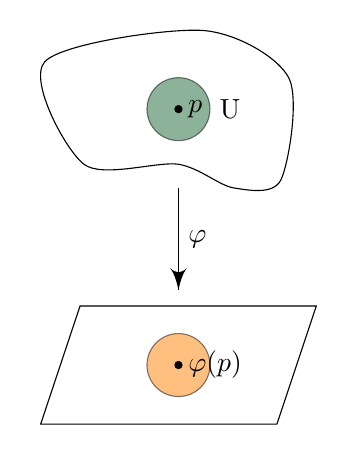
\begin{tikzpicture}
    \draw plot [smooth cycle] coordinates {(-1.2, -0.7) (0, -0.7) (0.7, -1) (1.3, -0.9) (1.4, 0.4) (0.3, 1) (-1.7, 0.6)};

    \draw [fill=mgreen, opacity=0.5] circle [radius=0.4];
    \node [right] {$p$};
    \node [circ] {};
    \node at (0.4, 0) [right] {U};

    \begin{scope}[shift={(-1.75, -4)}]
      \draw (0, 0) -- (3, 0) -- (3.5, 1.5) -- (0.5, 1.5) -- cycle;

      \draw (1.75, 0.75) [fill=morange, opacity=0.5] circle [radius=0.4];
      \node at (1.75, 0.75) [right] {$\varphi(p)$};
      \node at (1.75, 0.75) [circ] {};
    \end{scope}

    \draw [->] (0, -1) -- +(0, -1.3) node [pos=0.5, right] {$\varphi$};
  \end{tikzpicture}
\end{center}

\begin{defi}[Smooth function]\index{smooth function}\index{$C^\infty$}
  Let $(U, \varphi)$ be a chart on $M$, and $f: M \to \R$, we say $f$ is \emph{smooth} or $C^\infty$ at $p \in U$ if $f \circ \varphi^{-1}: \varphi(U) \to \R$ is smooth at $\varphi(p)$ in the usual sense.
  \[
    \begin{tikzcd}
      \R^n \supseteq \varphi(U) \ar[r, "\varphi^{-1}"] & U \ar[r, "f"] & \R
    \end{tikzcd}
  \]
\end{defi}
We can define all other notions such as continuity, differentiability, twice differentiability etc. similarly.

This definition has a problem that some points might not be in the chart, and we don't know how to determine if a function is, say, smooth at the point. The solution is easy --- we just take many charts that together cover $M$. However, we have the problem that a function might be smooth at a point relative to some chart, but not relative to some other chart. The solution is to require the charts to be compatible in some sense.

\begin{defi}[Atlas]\index{atlas}
  An \emph{atlas} on a set $M$ is a collection of charts $\{(U_\alpha, \varphi_\alpha)\}$ on $M$ such that
  \begin{enumerate}
    \item $M = \bigcup_{\alpha} U_\alpha$.
    \item For all $\alpha, \beta$, we have $\varphi_\alpha(U_\alpha \cap U_\beta)$ is open in $\R^n$, and the transition function
      \[
        \varphi_\alpha \circ \varphi_\beta^{-1}: \varphi_\beta(U_\alpha \cap U_\beta) \to \varphi_\alpha(U_\alpha \cap U_\beta)
      \]
      is smooth (in the usual set).
  \end{enumerate}
\end{defi}
\begin{center}
  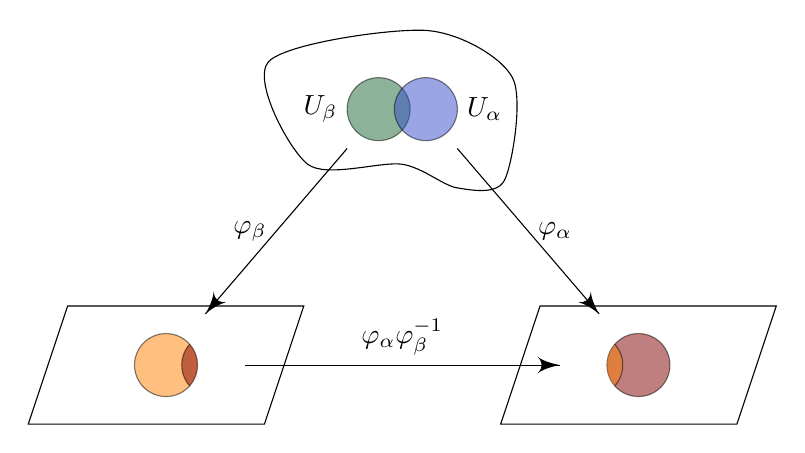
\begin{tikzpicture}
    \draw plot [smooth cycle] coordinates {(-1.2, -0.7) (0, -0.7) (0.7, -1) (1.3, -0.9) (1.4, 0.4) (0.3, 1) (-1.7, 0.6)};

    \draw (-0.3, 0) [fill=mgreen, opacity=0.5] circle [radius=0.4];
    \draw (0.3, 0) [fill=mblue, opacity=0.5] circle [radius=0.4];

    \node [left] at (-0.7, 0) {$U_\beta$};
    \node [right] at (0.7, 0) {$U_\alpha$};

    \begin{scope}[shift={(-4.75, -4)}]
      \draw (0, 0) -- (3, 0) -- (3.5, 1.5) -- (0.5, 1.5) -- cycle;

      \draw (1.75, 0.75) [fill=morange, opacity=0.5] circle [radius=0.4];
      \begin{scope}
        \clip (1.75, 0.75) circle [radius=0.4];
        \draw (2.35, 0.75) [fill=mred, opacity=0.5] circle [radius=0.4];
      \end{scope}
    \end{scope}

    \draw [->] (-0.7, -0.5) -- (-2.5, -2.6) node [pos=0.5, left] {$\varphi_\beta$};
    \draw [->] (0.7, -0.5) -- (2.5, -2.6) node [pos=0.5, right] {$\varphi_\alpha$};

    \begin{scope}[shift={(1.25, -4)}]
      \draw (0, 0) -- (3, 0) -- (3.5, 1.5) -- (0.5, 1.5) -- cycle;

      \draw (1.75, 0.75) [fill=mred, opacity=0.5] circle [radius=0.4];
      \begin{scope}
        \clip (1.75, 0.75) circle [radius=0.4];
        \draw (1.15, 0.75) [fill=morange, opacity=0.5] circle [radius=0.4];
      \end{scope}
    \end{scope}
    \draw [->] (-2, -3.25) -- (2, -3.25) node [pos=0.5, above] {$\varphi_\alpha \varphi_\beta^{-1}$};
  \end{tikzpicture}
\end{center}

\begin{lemma}
  If $(U_\alpha, \varphi_\alpha)$ and $(U_\beta, \varphi_\beta)$ are charts in some atlas, and $f: M \to \R$, then $f \circ \varphi_\alpha^{-1}$ is smooth at $\varphi_\alpha(p)$ if and only if $f \circ \varphi_\beta^{-1}$ is smooth at $\varphi_\beta (p)$ for all $p \in U_\alpha \cap U_\beta$.
\end{lemma}

\begin{proof}
  We have
  \[
    f \circ \varphi_\beta^{-1} = f \circ \varphi_\alpha^{-1} \circ (\varphi_\alpha \circ \varphi_\beta^{-1}).
  \]
\end{proof}

\begin{eg}
  Consider the sphere
  \[
    S^2 = \{(x_1, x_2, x_2): \sum x_i^2 = 1\} \subseteq \R^3.
  \]
  We let
  \[
    U_1^+ = S^2 \cap \{x_1 > 0\},\quad U_1^- = S^2 \cap \{x_1 < 0\}, \cdots
  \]
  We then let
  \begin{align*}
    \varphi_1^+: U_1^+ &\to \R^2\\
    (x_1, x_2, x_3) &\mapsto (x_2, x_3).
  \end{align*}
  It is easy to show that gives a bijection to the open disk in $\R^3$. We similarly define the other $\phi_i^{\pm}$. These then give us an atlas of $S^2$.
\end{eg}

\begin{defi}[Equivalent atlases]\index{equivalent atlases}\index{atlas!equivalence}
  Two atlases $\mathcal{A}_1$ and $\mathcal{A}_2$ are \emph{equivalent} if $\mathcal{A}_1 \cup \mathcal{A}_2$ is an atlas.
\end{defi}

\begin{defi}[Differentiable structure]\index{differentiable structure}
  A \emph{differentiable structure} on $M$ is a choice of equivalence class of atlases.
\end{defi}

We want to define a manifold to be a set with a differentiable structure. However, we still have the problem of giving it a topology. It turns out the smooth structure already gives us a topology.

\begin{ex}
  An atlas determines an topology on $M$ be saying $V \subseteq M$ is open iff $\varphi(U \cap V)$ is open in $\R^n$ for all charts $(U, \varphi)$ in the atlas. Equivalent atlases give the same topology.
\end{ex}

We now get to the definition of a manifold.

\begin{defi}[Manifold]\index{manifold}
  A \emph{manifold} is a set $M$ with a choice of differentiable structure whose topology is
  \begin{enumerate}
    \item Hausdorff\index{Hausdorff}, ie. for all $x, y \in M$, there are open neighbourhoods $U_x, U_y \subseteq M$ with $x \in U_x, y \in U_y$ and $U_x \cap U_y = \emptyset$.
    \item Second countable\index{second countable}, ie. there exists a countable collection $(U_n)_{n \in \N}$ of open sets in $M$ such that for all $V \subseteq M$ open, and $p \in V$, there is some $n$ such that $p \in U_n \subseteq V$.
  \end{enumerate}
\end{defi}
These requirements are there just to make sure we do not have pathological spaces. For example, the Hausdorff condition excludes the line with two origins from being a manifold, and the second countability condition excludes the long line. We will not use the second countability condition much.

Note that we will often refer to a manifold simply as $M$, where the differentiable structure is understood from context. By a chart on $M$, we mean one in some atlas in the equivalence class of atlases.

Say $\varphi: U \to \varphi(U) \subseteq \R^n$ is a chart of $M$. We think of $\varphi$ as $\varphi = (x_1, \cdots, x_n)$, with $x_i: U \to \R$. We call the $x_i$ the \emph{local coordinates}\index{local coordinates}. By abuse of notation, if $f: M \to \R$, we confuse $f|_U$ and $f \circ \varphi^{-1}: \varphi(U) \to \R$. So we write $f(x_1, \cdots, x_n)$ to mean $f(p)$, where $\varphi(p) = (x_1, \cdots, x_n) \in \varphi(U)$.
\[
  \begin{tikzcd}
    U \ar[r, hook, "\iota"] \ar[d, "\varphi"] & M \ar[r, "f"] & \R\\
    \varphi(U) \ar[rru, "f|_U"']
  \end{tikzcd}
\]
Of course, we can similarly define $C^0, C^1, C^2, \cdots$ manifolds, or analytic manifolds. We can also model manifolds on other spaces, eg. $\C^n$, where we get complex manifolds, or on infinite-dimensional spaces.

\begin{eg}\leavevmode
  \begin{enumerate}
    \item Generalizing the example of the sphere, the $n$-dimensional sphere $S^n = \{(x_0, \cdots, x_n) \in \R^{n + 1}: \sum x_i^2 = 1\}$ is a manifold.
    \item If $M$ is open in $\R^n$, then the inclusion map $\varphi: M \to \R^n$ given by $\varphi(p) = p$ is a chart forming an atlas. So $M$ is a manifold. In particular, $\R^n$ is a manifold, with its ``standard'' differentiable structure. We will always assume $\R^n$ is given this structure, unless otherwise specified.
    \item $M(n, n)$, the set of all $n \times n$ matrices is also a manifold, by the usual bijection with $\R^{n^2}$. Then $\GL_n \subseteq M(n, n)$ is open, and thus also a manifold.
    \item The set $\RP^n$, the set of one-dimensional subspaces of $\R^{n + 1}$ is a manifold. We can define charts as follows: we let $U_i$ to be the lines spanned by a vector of the form $(v_0, v_1, \cdots, v_{i - 1}, 1, v_{i + 1}, \cdots, v_n) \in \R^n$.

      We define the map $\varphi_i: U_i \to \R^n \cong \{\mathbf{x} \in \R^{n + 1}: x_i = 1\}$ that sends $\varphi(L) = (v_0, \cdots, 1, \cdots, v_n)$, where $L$ is spanned by $(v_0, \cdots, 1, \cdots, v_n)$. It is an easy exercise to show that this defines a chart.
  \end{enumerate}
\end{eg}

Note that when we defined a chart, we talked about charts as maps $U \to \R^n$. We did not mention whether $n$ is fixed, or whether it is allowed to vary. It turns out it cannot vary, as long as the space is connected.

\begin{lemma}
  Let $M$ be a manifold, and $\varphi_1: U_1 \to \R^n$ and $\varphi_2: U_2 \to \R^m$ be charts. If $U_1 \cap U_2 \not= \emptyset$, then $n = m$.
\end{lemma}

\begin{proof}
  We have $\varphi_1 \varphi_2^{-1}: \varphi_2(U_1 \cap U_2) \to \varphi_1(U_1 \cap U_2)$ is a smooth map with inverse $\varphi_2 \varphi_1^{-1}$. So $D(\varphi_1 \varphi_2^{-1})(\varphi(p)): \R^m \to \R^n$ is a linear isomorphism, whenever $p \in U_1 \cap U_2$. So $n = m$.
\end{proof}

\begin{defi}[Dimension]\index{dimension}
  If $p \in M$, we say $M$ has \emph{dimension} $n$ at $p$ if for one (thus all) charts $\varphi: U \to \R^m$ with $p \in U$, we have $m = n$. We say $M$ has dimension $n$ if it has dimension $n$ at all points.
\end{defi}

\section{Smooth functions and derivatives}
From now on, $M$ and $N$ will be manifolds.

\begin{defi}[Smooth function]\index{smooth function}
  A function $f: M \to N$ is \emph{smooth at a point $p \in M$} if there are charts $(U, \varphi)$ for $M$ and $(V, \zeta)$ for for $N$ with $p \in U$ and $f(p) \in V$ such that $\zeta \circ f \circ \varphi^{-1}: \varphi(U) \to \zeta(V)$ is smooth at $\varphi(p)$.

  A function is \emph{smooth} if it is smooth at all points $p \in M$.

  A \term{diffeomorphism} is a smooth $F$ with a smooth inverse.

  We write $C^\infty(M, N)$ \index{$C^\infty(M, N)$} for the space of smooth maps $F: M \to N$. We write $C^\infty(M)$\index{$C^\infty(M)$} for $C^\infty(M, \R)$, and this has the additional structure of an algebra, ie. vector space with multiplication.
\end{defi}
\begin{center}
  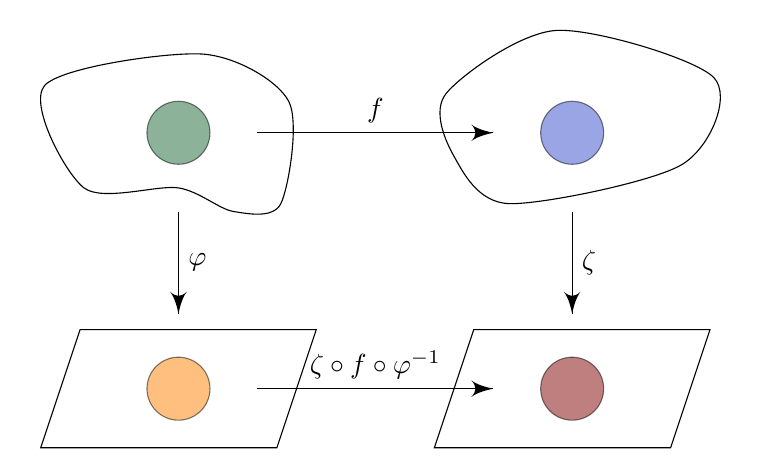
\begin{tikzpicture}
    \draw plot [smooth cycle] coordinates {(-1.2, -0.7) (0, -0.7) (0.7, -1) (1.3, -0.9) (1.4, 0.4) (0.3, 1) (-1.7, 0.6)};

    \draw [fill=mgreen, opacity=0.5] circle [radius=0.4];

    \begin{scope}[shift={(-1.75, -4)}]
      \draw (0, 0) -- (3, 0) -- (3.5, 1.5) -- (0.5, 1.5) -- cycle;

      \draw (1.75, 0.75) [fill=morange, opacity=0.5] circle [radius=0.4];
    \end{scope}

    \draw [->] (0, -1) -- +(0, -1.3) node [pos=0.5, right] {$\varphi$};
    \begin{scope}[shift={(5, 0)}]
      \draw plot [smooth cycle] coordinates {(1.4, -0.4) (-0.8, -0.9) (-1.5, -0.3) (-1.6, 0.5) (-0.2, 1.3) (1.8, 0.7)};

      \draw [fill=mblue, opacity=0.5] circle [radius=0.4];

      \begin{scope}[shift={(-1.75, -4)}]
        \draw (0, 0) -- (3, 0) -- (3.5, 1.5) -- (0.5, 1.5) -- cycle;

        \draw (1.75, 0.75) [fill=mred, opacity=0.5] circle [radius=0.4];
      \end{scope}

      \draw [->] (0, -1) -- +(0, -1.3) node [pos=0.5, right] {$\zeta$};
    \end{scope}

    \draw [->] (1, 0) -- (4, 0) node [above, pos=0.5] {$f$};

    \draw [->] (1, -3.25) -- (4, -3.25) node [above, pos=0.5] {$\zeta \circ f \circ \varphi^{-1}$};
  \end{tikzpicture}
\end{center}
Equivalently, $f$ is smooth at $p$ if $\zeta \circ F \circ \varphi^{-1}$ is smooth at $\varphi(p)$ for \emph{any} such charts $(U, \varphi)$ and $(V, \zeta)$.

\begin{eg}
  Let $\varphi: U \to \R^n$ be a chart. Then $\varphi: U \to \varphi(U)$ is a diffeomorphism.
\end{eg}

\begin{defi}[Curve]\index{curve}
  A \emph{curve} is a smooth map $I \to M$, where $I$ is a non-empty open interval.
\end{defi}

To discuss derivatives, we first look at the case where $U \subseteq \R^n$ is open. Suppose $f: U \to \R$ is smooth. If $p \in U$ and $v \in \R^n$, recall that the \term{directional derivative} is defined by
\[
  Df|_p(v) = \lim_{t \to 0} \frac{f(p + t\mathbf{v}) - f(p)}{t}.
\]
If $\mathbf{v} = \mathbf{e}_i = (0, \cdots, 1, 0, \cdots, 0)$, then we write
\[
  Df|_p (\mathbf{e}_i) = \left.\frac{\partial f}{\partial x_i}\right|_p.
\]
Also, we know $Df|_p: \R^n \to \R$ is a linear map (by definition of smooth).

Note that here $p$ and $\mathbf{v}$ are both vectors, but they play different roles --- $p$ is an element in the domain $U$, while $\mathbf{v}$ is an arbitrary vector in $\R^n$. Even if $\mathbf{v}$ is enormous, by taking a small enough $t$, we find that $p + t\mathbf{v}$ will eventually be inside $U$.

If we have a general manifold, we can still talk about the $p$. However, we don't have anything that plays the role of a vector. Our first goal is to define the tangent space to a manifold that captures where the ``directions'' live.

An obvious way to do so would be to use a curve. Suppose $\gamma: I \to M$ is a curve, with $\gamma(0) = p \in U \subseteq M$, and $f: U \to \R$ is smooth. We can then take the derivative of $f$ along $\gamma$ as before. We let
\[
  X(f) = \left.\frac{\d}{\d t}\right|_{t = 0} f(\gamma(t)).
\]
It is an exercise to see that $X: C^\infty(U) \to \R$ is a linear map, and it satisfies the \term{Leibnitz rule}
\[
  X(fg) = f(p) X(g) + g(p) X(f).
\]
We denote $X$ by $\dot{\gamma}(0)$. We might think of defining the tangent space as curves up to some equivalence relation, but if we do this, there is no obvious vector space on it. However, if we define a tangent vector as a linear map satisfying the Leibnitz rule, then it has an automatic, obvious vector space structure.
\begin{defi}[Derivation]\index{derivation}
  A \emph{derivation} on an open subset $U \subseteq M$ at $p \in U$ is a linear map $X: C^\infty(U) \to \R$ satisfying the Leibnitz rule
  \[
    X(fg) = f(p) X(g) + g(p) X(f).
  \]
\end{defi}

\begin{defi}[Tangent space]\index{tangent space}
  Let $p \in U \subseteq M$, where $U$ is open. The \emph{tangent space} of $M$ at $p$ is the vector space
  \[
    T_p(M) = \{\text{derivations on $U$ at $p$}\}.
  \]
  The subscript $p$ tells us the point at which we are taking the tangent space.
\end{defi}
We will later show that this does not depend on $U$. It is easy to see that if $\gamma: i \to M$ is a curve with $\gamma(0) = p$, then $\dot{\gamma}(0) = T_p(M)$. We will also later show that all derivations do come from some path, which is less trivial.

\begin{eg}
  Let $U \subseteq \R^n$ be open, and let $p \in U$. Let $D_{e_i, q} \in T_q \R^n$ be
  \[
    D_{e_i, q} = \left.\frac{\partial f}{\partial x_i}\right|_q.
  \]
\end{eg}

\begin{lemma}
  $\{D_{e_1, q}, \cdots, D_{e_n, q}\}$ is a basis of $T_q \R^n$. So these are all the derivations.
\end{lemma}

The idea of the proof is to show that a derivation can only depend on the first order derivatives of a function, and all possibilities will be covered by the $D_{e_i, q}$.

\begin{proof}
  Independence is clear as
  \[
    D_{e_i, q}(x_j) = \frac{\partial x_j}{\partial x_i} = \delta_{ij}.
  \]
  We need to show spanning. For notational convenience, we wlog $q = 0$. Let $X \in T_0 \R^n$.

  We first show that if $g \in C^\infty(U)$ is the constant function $g = 1$, then $X(g) = 0$. Indeed, we have
  \[
    X(g) = X(g^2) = g(0) X(g) + X(g) g(0) + 2 X(g).
  \]
  Thus, if $h$ is any constant function, say, $c$, then $X(h) = X(cg) = c X(g)$. So the derivative of any constant function vanishes.

  In general, let $f \in C^\infty(U)$. By Taylor's theorem, we have
  \[
    f(x_1, \cdots, x_n) = f(0) + \sum \frac{\partial f}{\partial x_i} x_i + \varepsilon,
  \]
  where $\varepsilon$ is a sum of terms of the form $x_i x_j h$ with $h \in C^\infty(U)$.

  We set $\lambda_i = X(x_i) \in \R$. We first claim that $X(\varepsilon) = 0$. Indeed, we have
  \[
    X (x_i x_j h) = x_i|_{0} X(x_j h) + (x_jh)(0) X(x_i) = 0.
  \]
  So we have
  \[
    X(f) = \sum \lambda_i \left.\frac{\partial f}{\partial x_i}\right|_0.
  \]
  So we have
  \[
    X = \sum \lambda_i D_{e_i, q}.
  \]
\end{proof}

\begin{defi}[Derivative]\index{derivative}
  Suppose $F \in C^\infty(M, N)$, say $F(p) = q$. We define $\D F|_p: T_p M \to T_q N$ by
  \[
    \D F|_p(X)(g) = X(g \circ F)
  \]
  for $X \in T_pM$ and $g \in C^\infty(V)$ with $q \in V \subseteq N$.

  This is a linear map called the \emph{derivative} of $F$ at $p$.
\end{defi}

\begin{prop}[Chain rule]\index{chain rule}
  Let $M, N, P$ be manifolds, and $F \in C^\infty(M, N)$, $G \in C^\infty(N, P)$, and $p \in M, q \in F(p)$. Then we have
  \[
    \D(G \circ F)|_p = \D G|_q \circ \D F|_p.
  \]
\end{prop}

\begin{proof}
  We have
  \[
    (\D F|_p (X))(h) = \D F|_p(X) (h \circ G) = X(h \circ G \circ F) = \D (G \circ F)|_p (X).
  \]
\end{proof}

\begin{cor}
  If $F$ is a diffeomorphism, then $\D F|_p$ is a linear isomorphism, and $(\D F|_p)^{-1} = \D (F^{-1})|_{F(p)}$.
\end{cor}

We now go back to understanding what $T_pM$ is if $p \in M$. We let $p \in U$ where $(U, \varphi)$ be a chart. Then if $q = \varphi(p)$, then $D\varphi|_p: T_p M \to T_q \R^n$ is a linear isomorphism.

\begin{defi}[$\frac{\partial}{\partial x_i}$]\index{$\frac{\partial}{\partial x_i}$}
  Given a chart $\varphi: U \to \R^n$ with $\varphi = (x_1, \cdots, x_n)$, we define
  \[
    \left.\frac{\partial}{\partial x_i}\right|_p = (D \varphi|_p)^{-1} (D_{e_i, q}) \in T_p M.
  \]
\end{defi}
So $\left.\frac{\partial}{\partial x_1}\right|_p, \left.\frac{\partial}{\partial x_2}\right|_p, \cdots$ are a basis for $T_p M$.

Recall that if $f: U \to \R$ is smooth, we write $f(x_1, \cdots, x_n)$. Then we have
\[
  \left.\frac{\partial}{\partial x_i}\right|_p (f) = \left.\frac{\partial f}{\partial x_i}\right|_{\varphi(p)}.
\]
So we have a consistent notation.

Now how does this basis change when we change coordinates? Suppose we also have coordinates $y_1, \cdots, y_n$ near $p$ given by some other chart. We then have $\left.\frac{\partial}{\partial y_i}\right|_p \in T_p M$. So we have
\[
  \left.\frac{\partial}{\partial y_i}\right|_p = \sum_j \alpha_j \left.\frac{\partial}{\partial x_j}\right|_p
\]
for some $\alpha_j$. To figure out what they are, we apply them to the function $x_k$. So we have
\[
  \left.\frac{\partial x_k}{\partial y_i}\right|_p = \alpha_k.
\]
So we obtain
\[
  \frac{\partial}{\partial y_i} = \sum_j \frac{\partial x_j}{\partial y_i} \frac{\partial}{\partial x_j}.
\]
This is the usual change-of-coordinate formula!

Now recall that if $F \in C^\infty (M, N)$ with $F(p) = q$, then we obtain a linear map $\D F|_p: T_pM \to T_q N$ given by
\[
  \D F|_p(X)(g) = X(g \circ F)
\]
for $X \in T_p(M)$ and $g \in C^\infty (V, \R)$.

Now suppose $(U, \varphi)$ is a chart on $M$ containing $p$ with coordinates $x_1, \cdots, x_n$, and $(V, \zeta)$ is a chart on $N$ containing $q$ with coordaintes $y_1,\cdots, y_m$.

By abuse of notation, we confuse $F$ and $\zeta \circ F \circ \varphi^{-1}$. So we write $F = (F_1, \cdots, F_n)$ with $F_i = F_i(x_1, \cdots, x_n): U \to \R$.

As before, we have a basis
\begin{align*}
  \left.\frac{\partial}{\partial x_i}\right|_p, \cdots, \left.\frac{\partial}{\partial x_n}\right|_p&\quad\text{for}\quad T_pM,\\
  \left.\frac{\partial}{\partial y_i}\right|_q, \cdots, \left.\frac{\partial}{\partial y_m}\right|_q&\quad\text{for}\quad T_qN.
\end{align*}

\begin{lemma}
  We have
  \[
    \D F|_p \left(\left.\frac{\partial}{\partial x_i}\right|_p\right) = \sum_{j = 1}^n \frac{\partial F_j}{\partial x_i}(p) \left.\frac{\partial}{\partial y_j}\right|_p.
  \]
  In other words, $\D F|_p$ has matrix representation
  \[
    \left(\frac{\partial F_j}{\partial x_i}(p)\right)_{ij}.
  \]
\end{lemma}

\begin{proof}
  We let
  \[
    \D F|_p \left(\left.\frac{\partial}{\partial x_i}\right|_p\right) = \sum_{j = 1}^n \lambda_j \left.\frac{\partial}{\partial y_j}\right|_p.
  \]
  for some $\lambda_i$. We apply this to the local function $y_k$ to obtain
  \begin{align*}
    \lambda_k &= \left(\sum \lambda_j \left.\frac{\partial}{\partial y_j}\right|_p\right)(y_k)\\
    &= \D F_p \left(\left.\frac{\partial}{\partial x_i}\right|_p\right)(y_k)\\
    &= \left.\frac{\partial}{\partial x_i}\right|_p (y_k \circ F) = \left.\frac{\partial}{\partial x_i}\right|_p(F_k) = \frac{\partial F_k}{\partial x_i}(p).
  \end{align*}
\end{proof}

\begin{eg}
  Let $f: C^\infty(U)$ where $U \subseteq M$ is an open set containing $p$. Then $\D f|_p: T_p M \to T_{f(p)} \R \cong \R$ is a linear map. So $\D f|_p$ is an element in the dual space $(T_pM)^*$, called the \term{differential} of $f$ at $p$, and is denoted $\d f|_p$.
\end{eg}

Recall that there is one thing we swept under the carpet --- to define the tangent space, we needed to pick an open set $U$. Ways to deal with this can be found in the example sheet, but there are two general approaches --- one is to talk about germs of functions, where we consider all open neighbourhoods, and identify two functions if they agree on some open neighbourhood of the point. The other way is to realize that we can ``extend'' any function on $U \subseteq M$ to a function on the whole of $M$, using bump functions.

In general, we want a function that looks like this:
\begin{center}
  \begin{tikzpicture}
    \draw [->] (-3, 0) -- (3, 0);
    \draw [->] (0, -0.5) -- (0, 3);
    \draw [thick, blue] (-1.01, 2) -- (1.01, 2);
    \draw [thick, blue] (-3, 0) -- (-1.99, 0);
    \draw [thick, blue] (1.99, 0) -- (3, 0);
    \draw [domain=-1.99:-1.01, thick, blue] plot [smooth] (\x, {2 * (exp(- 1 / ((2 + \x) * (2 + \x))))/((exp(- 1 / ((2 + \x) * (2 + \x)))) + (exp(- 1 / ((-1 - \x) * (-1 - \x)))))});
    \draw [domain=1.01:1.99, thick, blue] plot [smooth] (\x, {2 * (exp(- 1 / ((2 - \x) * (2 - \x))))/((exp(- 1 / ((2 - \x) * (2 - \x)))) + (exp(- 1 / ((-1 + \x) * (-1 + \x)))))});
  \end{tikzpicture}
\end{center}

\begin{lemma}
  Suppose $W \subseteq M$ is a coordinate chart with $p \in W$. then there is an open neighbourhood $V$ of $p$ such that $\bar{V} \subseteq W$ and an $X \in C^\infty(M, \R)$ such that $x = 1$ on $V$ and $W = 0$ on $M \setminus W$.
\end{lemma}

\begin{proof}
  Suppose we have coordiantes $x_1, \cdots, x_n$ on $W$. We wlog suppose these are defined for all $|x| < 3$.

  We define $\alpha, \beta, \gamma: \R \to \R$ by
  \[
    \alpha(t) =
    \begin{cases}
      e^{-t^{-2}} & t > 0\\
      0 & t \leq 0
    \end{cases}.
  \]
  \begin{center}
    \begin{tikzpicture}
      \draw [->] (-3, 0) -- (3, 0);
      \draw [->] (0, -0.5) -- (0, 3);
      \draw [thick, blue] (-3, 0) -- (0, 0);
      \draw [domain=0.01:3, thick, blue] plot [smooth] (\x, {2 * exp(- 1 / (\x * \x))});
    \end{tikzpicture}
  \end{center}
  We now let
  \[
    \beta(t) = \frac{\alpha(t)}{\alpha(t) + \alpha(1 - t)}.
  \]
  \begin{center}
    \begin{tikzpicture}[xscale=4]
      \draw [->] (0, 0) -- (1, 0);
      \draw [->] (0, -0.5) -- (0, 3);
      \draw [thick, blue] (0, 0) -- (0.01, 0);
      \draw [domain=0.01:0.99, thick, blue] plot [smooth] (\x, {2 * (exp(- 1 / (\x * \x)))/((exp(- 1 / (\x * \x))) + (exp(- 1 / ((1 - \x) * (1 - \x)))))});
    \end{tikzpicture}
  \end{center}
  Then we let
  \[
    \gamma(t) = \beta(t + 2)\beta(2 - t).
  \]
  \begin{center}
    \begin{tikzpicture}
      \draw [->] (-3, 0) -- (3, 0);
      \draw [->] (0, -0.5) -- (0, 3);
      \draw [thick, blue] (-1.01, 2) -- (1.01, 2);
      \draw [thick, blue] (-3, 0) -- (-1.99, 0);
      \draw [thick, blue] (1.99, 0) -- (3, 0);
      \draw [domain=-1.99:-1.01, thick, blue] plot [smooth] (\x, {2 * (exp(- 1 / ((2 + \x) * (2 + \x))))/((exp(- 1 / ((2 + \x) * (2 + \x)))) + (exp(- 1 / ((-1 - \x) * (-1 - \x)))))});
      \draw [domain=1.01:1.99, thick, blue] plot [smooth] (\x, {2 * (exp(- 1 / ((2 - \x) * (2 - \x))))/((exp(- 1 / ((2 - \x) * (2 - \x)))) + (exp(- 1 / ((-1 + \x) * (-1 + \x)))))});
    \end{tikzpicture}
  \end{center}
  Finally, we let
  \[
    X(x_1, \cdots, x_n) = \gamma(x_1) \cdots \gamma(x_n).
  \]
  on $W$. We let
  \[
    V = \{\mathbf{x}: |x_i| < 1\}.
  \]
  Extending $X$ to be identically $0$ on $M \setminus W$ to get the desired smooth function (up to some constant).
\end{proof}
\begin{lemma}
  Let $p \in W \subseteq U$ and $W, U$ open. Let $f_1, f_2 \in C^\infty(U)$ be such that $f_1 = f_2$ on $W$. Then if $X \in \Der_p(C^\infty(U))$, then we have $X(f_1) = X(f_2)$
\end{lemma}

\begin{proof}
  Set $h = f_1 - f_2$. We can wlog $W$ is a coordinate chart. We pick a bump function $\chi \in C^\infty(U)$ that vanishes outside $W$. Then $\chi h = 0$. Then we have
  \[
    0 = X(\chi h) = \chi(p) X(h) + h(p) X(\chi) = X(h) + 0 = X(f_1) - X(f_2).
  \]
\end{proof}

\section{Submanifolds}
You have a manifold, and a subset of it is a manifold, so you call it a submanifold. Except there are some subtleties here. There will be two kinds of submanifolds we can talk about, namely embedded submanifolds and immersed submanifold.

\begin{defi}[Embedded submanifold]\index{Embedded submanifold}
  Let $M$ be a manifold with $\dim M = n$, and $S$ be a submanifold of $M$. We say $S$ is an \emph{embedded manifold} if for all $p \in S$, there are coordinates $x_1, \cdots, x_n$ on some chart $U \subseteq M$ containing $p$ such that
  \[
    S \cap U = \{x_{k + 1} = x_{k + 2} = \cdots = x_n = 0\}.
  \]
  Such coordinates are known as \term{slice coordinates} for $S$.
\end{defi}

\begin{lemma}
  If $S$ is an embedded submanifold of $M$, then there exists a unique differential structure on $S$ such that the inclusion map $\iota: S \hookrightarrow M$ is smooth, and $S$ inherits the subspace topology.
\end{lemma}

\begin{proof}
  Basically if $x_1, \cdots, x_n$ is a slice chart for $S$ in $M$, then $x_1, \cdots, x_k$ will be coordinates on $S$.

  More precisely, let $\pi: \R^n \to \R^k$ be the projection map
  \[
    \pi(x_1, \cdots, x_n) = (x_1, \cdots, x_k).
  \]
  Given a slice chart $(U, \varphi)$ for $S$ in $M$, consider $\tilde{\varphi}: S \cap U \to \R^k$ by $\tilde{\varphi} = \pi \circ \varphi$. This is smooth and bijective, and is so a chart on $S$. These cover $S$ by assumption. So we only have to check that the transition functions are smooth.

  Given another slice chart $(V, \zeta)$ for $S$ in $M$, we let $\tilde{\zeta} = \pi \circ \zeta$, and check that
  \[
    \tilde{\zeta} \circ \tilde{\varphi}^{-1} = \pi \circ \zeta \circ \varphi^{-1} \circ j,
  \]
  where $j: \R^k \to \R^n$ is given by $j(x_1, \cdots, x_k) = (x_1, .., x_k, 0, \cdots, 0)$.

  From this characterization, by looking at local charts, it is clear that $S$ has the subspace topology. It is then easy to see that the embedded submanifold is Hausdorff and second-countable, since these properties are preserved by taking subspaces.

  We can also check easily that $\iota: S\to M$ is smooth, and this is the only differential structure with this property.
\end{proof}

It is also obvious from the slice charts that
\begin{prop}
  Let $S$ be an embedded submanifold. Then the derivative of the inclusion map $i: S \to M$ is injective.
\end{prop}

If we drop everything else and only keep this condition, we get the notion of an immersed manifold.

\begin{defi}[Immersed submanifold]\index{immersed submanifold}
  Let $S, M$ be manifolds, and $i: S \to M$ be a smooth injective map with $Di|_p : T_p S \to T_p M$ is injective for all $p \in S$. Then we call $(i,, S)$ an \emph{immersed submanifold}. By abuse, we identify $S$ and $i(S)$.
\end{defi}

\begin{eg}
  If we map $\R$ into $\R^2$ via the following figure of eight (where the arrow heads denote the ``end points'' of $\R$), then this gives an immersed manifold that is not an embedded manifold.
  \begin{center}
    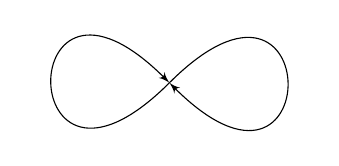
\begin{tikzpicture}
      \path[use as bounding box] (-1.8, -0.7) rectangle (1.8,0.7);
      \draw [-latex'] (0, 0) .. controls (2, 2) and (2, -2) .. (0, 0);
      \draw [-latex'] (0, 0) .. controls (-2, -2) and (-2, 2) .. (0, 0);
    \end{tikzpicture}
  \end{center}
\end{eg}

\begin{eg}
  Consider the line $\R$, and define the map $f: \R \to T^2 = \R^2 / \Z^2$ by $f(x) = \alpha x$, where $\alpha$ is some irrational number. Then this map gives an immersed submanifold of $T^2$, but is not an embedded submanifold, since $\R$ certainly does not have the subspace topology from $T^2$.
\end{eg}

\begin{defi}[Regular value]\index{regular value}
  Let $F \in C^\infty(M, N)$ and $c \in N$. Let $S = F^{-1}(c)$. We say $c$ is a \emph{regular value} if for all $p \in S$, the map $\D F|_p: T_p M \to T_c N$ is surjective.
\end{defi}

\begin{prop}
  Let $F \in C^\infty(M, N)$, and let $c \in N$. Suppose $c$ is a regular value. Then $S = F^{-1}(c)$ is an embedded submanifold of dimension $\dim M - \dim N$.
\end{prop}

\begin{proof}
  We let $n = \dim M$ and $m = \dim N$. Notice that for the map $\D F$ to be surjective, we must have $n \geq m$.

  Let $p \in S$, so $F(p) = c$. We want to find a slice coordinate for $S$ near $p$. Since the problem is local, by restricting to local coordinate charts, we may wlog $N = \R^m$, $M = \R^n$ and $c = p = 0$.

  Thus, we have a smooth map $F: \R^n \to \R^m$ with surjective derivative at $0$. Then the derivative is
  \[
    \left(\left.\frac{\partial F_j}{\partial x_i}\right|\right)_{i = 1, \ldots, n; j = 1, \ldots, m},
  \]
  which by assumption has rank $m$. We reorder the $x_i$ so that the first $m$ columns are independent. Then the $m \times m$ matrix
  \[
    R = \left(\left.\frac{\partial F_j}{\partial x_i}\right|\right)_{i,j = 1, \ldots, m}
  \]
  is non-singular. We consider the map
  \[
    \alpha(x_1, \cdots, x_n) = (F_1, \cdots, F_n, x_{n + 1}, x_{n + 2}, \cdots, x_m).
  \]
  We then obtain
  \[
    \D \alpha|_0 =
    \begin{pmatrix}
      R & * \\
      0 & I
    \end{pmatrix},
  \]
  and this is non-singular. By the inverse function theorem, $\alpha$ is a local diffeomorphism. So there is an open $W\subseteq \R^n$ containing $0$ such that $\alpha|_W: W \to \alpha(W)$ is smooth with smooth inverse. We claim that $\alpha$ is a slice chart of $S$ in $\R^n$.

  Since it is a smooth diffeomorphism, it is certainly a chart. Moreover, by construction, the points in $S$ are exactly those whose image under $F$ have the first $n$ coordinates vanish. So this is the desired slice chart.
\end{proof}

\begin{eg}
  We want to show that $S^n$ is a manifold. Let $F: \R^{n + 1} \to \R$ be defined by
  \[
    F(x_0, \cdots, x_n) = \sum x_i^2.
  \]
  Then $F^{-1}(1) = S^n$. We find that
  \[
    \D F|_p = 2(x_0, \cdots, x_{n + 1}) \not= 0
  \]
  when $p \in S^n$. So $S^n$ is a manifold.
\end{eg}

\begin{eg}
  Consider the orthogonal group. We let $M_n \cong \R^{n^2}$ be the space of all $n \times n$ matrices with the obvious smooth structure. We define
  \[
    N = \{A \in M_n: A^T = A\}.
  \]
  Since this is a linear subspace, it is also a manifold. We define
  \begin{align*}
    F: M_n &\to N\\
    A &\mapsto AA^T.
  \end{align*}
  Then we have
  \[
    \Or(n) = F^{-1}(I) = \{A: AA^T = I\}.
  \]
  We compute the derivative by looking at
  \[
    F (A + H) = (A + H)(A + H)^T = AA^T + HA^T + AH^T + HH^T.
  \]
  So we have
  \[
    \D F|_n (H) = HA^T + AH^T.
  \]
  Now if $A \in \Or(A)$, then we have
  \[
    \D F|_A (HA) = HAA^T + AA^T H^T = H + H^T
  \]
  for any $H$. Since every symmetric matrix is of the form $H + H^T$, we know $\D F|_A: T_A M_n \to T_{F(A)}N$ is surjective. So $\Or(n)$ is a manifold.
\end{eg}

\section{Tangent bundle}
Recall that we had the notion of a tangent bundle. If we have a curve $\gamma: I \to M$, then we would like to think that the derivative $\dot{\gamma}$ ``varies smoothly'' with time. However, we cannot really do that yet, since for different $t$, the value of $\dot{\gamma}$ lies in different vector spaces, and there isn't a way of comparing them.

Alternatively, given a ``vector field'' $f: p \mapsto v_p \in T_p M$ for each $p \in M$, how do we ask if this is a smooth function?

One way to solve this is to pick local coordinates $x_1, \cdots,x _n$ on $U \subseteq M$. We can then write
\[
  v_p = \sum_k \alpha_i(p) \left.\frac{\partial}{\partial x_i}\right|_p.
\]
Since $\alpha_i(p) \in \R$, we can say $v_p$ varies smoothly if the functions $\alpha_i(p)$ are smooth. We then proceed to check that this does not depend on coordinates etc.

However, there is a more direct approach. We simply turn
\[
  TM = \bigcup_{p \in M} T_p M
\]
into a manifold. There is then a natural map $\pi: TM \to M$ sending $v_p \in p$ for each $v_p \in M$, and this is smooth. We can then define the smoothness of $v_p$ using the usual notion of smoothness of maps between manifolds.

\begin{defi}[Vector field]
  A \term{vector field} on some $U \subseteq M$ is a smooth map $X: u \to TM$ such that for all $p \in U$, we ahve
  \[
    X(p) \in T_p M.
  \]
  In other words, we have $\pi \circ X = \id$.
\end{defi}

\begin{defi}[$\Vect(U)$]\index{$\Vect(U)$}
  Let $\Vect(U)$ denote the set of all vector fields on $U$. Let $X, Y \in \Vect(U)$, and $f \in C^\infty(U)$. Then we can define
  \[
    (X + Y)(p) = X(p) + Y(p),\quad (fX)(p) = f(p) X(p).
  \]
  Then we have $X + Y, fX \in \Vect(U)$. So $\Vect(U)$ is a $C^\infty(U)$ module.

  Moreover, if $V \subseteq U \subseteq M$ and $X \in V=\Vect(U)$, then $X|_V \in \Vect(V)$.

  Conversely, if $\{V_i\}$ is a cover of $U$, and $X_i \in V_i$ are such that they agree on intersections, then they patch together to give an element of $\Vect(U)$. So we say that $\Vect$ is a \emph{sheaf of $C^\infty(M)$ modules}.
\end{defi}

Now we properly define the manifold structure on the tangent bundle.

\begin{defi}[Tangent bundle]\index{tangent bundle}
  Let $M$ be a manifold, and
  \[
    TM = \bigcup_{p \in M}T_p M.
  \]
  There is a natural projection map $\pi: TM \to M$ sending $v_p \in T_pM$ to $p$.

  Let $x_1, \cdots, x_n$ be coordinates on a chart $(U, \varphi)$. Then for any $p \in U$ and $v_p \in T_p M$, there is some $\alpha_1, \cdots, \alpha_n \in \R$ such that
  \[
    v_p = \sum_{i = 1}^n \alpha_i \left.\frac{\partial}{\partial x_i}\right|_{p}.
  \]
  This gives a map
  \[
    v_p \mapsto (x_1(p), \cdots, x_n(p), \alpha_1, \cdots, \alpha_n),
  \]
  which is a bijection
  \[
    \tilde{\varphi}: \pi^{-1}(U) = \bigcup_{p \in U} T_p(M) \to U \times \R^n.
  \]
  So $(\tilde{\varphi}, \pi^{-1}(U))$ is a chart on $TM$.

  These charts make $TM$ into a manifold of dimension $2 \dim M$, called the \emph{tangent bundle} of $M$.
\end{defi}

\begin{lemma}
  The charts actually make $TM$ into a manifold.
\end{lemma}

\begin{proof}
  If $V(, \xi)$ is another chart on $M$ with coordinates $y_1, \cdots, y_m$, then
  \[
    \left.\frac{\partial}{\partial x_i}\right|_p = \sum_j \frac{\partial y_j}{\partial x_i}(p) \left.\frac{\partial y_i}{\partial y_i}\right|_p.
  \]
  So we have $\tilde{\zeta} \circ \tilde{\varphi}^{-1}: \varphi(U \cap V) \times \R^n \to \zeta(U \cap V) \times \R^n$ given by
  \[
    \tilde{\zeta} \circ \tilde{\varphi}^{-1} (x_1, \cdots, x_n \alpha_1, \cdots, \alpha_n) = \left(y_1, \cdots, y_n, \sum_i \alpha_i \frac{\partial y_{n + 1}}{\partial x_i}, \cdots, \sum \alpha_i \frac{\partial y_n}{\partial x_i}\right),
  \]
  and is smooth (an in fact fiberwise linear).

  It is easy to check that $TM$ is Hausdorff and second countable as $M$ is.
\end{proof}

There are a few remarks to make about this.
\begin{enumerate}
  \item The projection map $\pi: TM \to M$ is smooth.
  \item If $U \subseteq M$ is open, recall that
    \[
      \Vect(U) = \{\text{smooth }X: U \to TM\mid X(p) \in T_pM\text{ for all }p \in U\}.
    \]
    We write $X_p$ for $X(p)$. Now suppose further that $U$ is a coordinate chart, then we can write any function $X: U \to T_p M$ such that $X_p \in T_p M$ (uniquely) as
    \[
      X_p = \sum \alpha_i(p) \left.\frac{\partial}{\partial x_i} \right|_p
    \]
    Then $X$ is smooth iff all $\alpha_i$ are smooth.
  \item If $F \in C^\infty(M, N)$, then $\D F: TM \to TN$ given by $\D F(v_p) = \D F|_p(v_p)$ is smooth. This is nice, since we can easily talk about higher derivatives, by taking the derivative of the derivative map.
  \item If $F \in C^\infty (M, N)$ and $X$ is a vector field on $N$, then we cannot obtain a vector field on $N$ by $\D F(X)$, since $F$ might not be injective. If $F(p_1) = F(p_2)$, we need not have $\D F(X(p_1)) = \D F(X(p_2))$.
\end{enumerate}
However, there is a weaker notion of being $F$-related.
\begin{defi}[$F$-related]\index{$F$-related}
  Let $M, N$ be manifolds, and $X \in \Vect(M)$, $Y \in \Vect(N)$ and $F \in C^\infty(M, N)$. We say they are \emph{$F$-related} if
  \[
    Y_q = \D F|_p (X_p)
  \]
  for all $p \in M$ and $F(p) = q$. In other words, if the following diagram commutes:
  \[
    \begin{tikzcd}
      TM \ar[r, "\D F"] & TN\\
      M \ar[u, "X"] \ar[r, "F"] & N \ar[u, "Y"]
    \end{tikzcd}.
  \]
\end{defi}

So what does $\Vect(M)$ look like? We start with an algebraic description of $\Vect(M)$. This is an $\R$-vector space, and in fact an $C^\infty(M)$ module. We let $\Der(C^\infty(M, \R))$ be the set of all derivations of all $\R$-linear maps $\mathcal{X}: C^\infty(M) \to C^\infty(M)$ that satisfies
\[
  \mathcal{X}(fg) = f \mathcal{X}(g) + \mathcal{X}(f) g.
\]
Given $X \in \Vect(M)$, we get a derivation $\mathcal{X} \in \Der(C^\infty(M, \R))$ by setting
\[
  \mathcal{X}(f)(p) = X_p(f).
\]
It is an exercise to show that $\mathcal{X}(f)$ is smooth and satisfies the Leibnitz rule. Similar to the case of vectors, we want to show that all derivations come from vector fields.

\begin{lemma}
  The map $X \mapsto \mathcal{X}$ is a $\R$-linear isomorphism
  \[
    \Gamma: \Vect(M) \to \Der(C^\infty(M, \R)).
  \]
\end{lemma}

\begin{proof}
  Suppose that $\alpha$ is a derivation. If $p \in m$, we define
  \[
    X_p(f) = \alpha(f)(p)
  \]
  for all $f \in C^\infty(M)$. This is certainly a linear map, and we have
  \[
    X_p(fg) = \alpha(fg)(p) = (f\alpha(g) + g\alpha(f))(p) = f(p) X_p(g) + g(p) X_p(f).
  \]
  So $X_p \in T_p M$. We just need to check that the map $M \to TM$ sending $p \mapsto X_p$ is smooth. Locally on $M$, we have coordinates $x_1, \cdots, x_n$, and we can write
  \[
    X_p = \sum \alpha_i(p) \left.\frac{\partial}{\partial x_i}\right|_p.
  \]
  We want to show that $\alpha_i: U \to \R$ are smooth.

  We pick a bump function $\varphi$ that is identically $1$ near $p$, with $\supp \varphi \subseteq U$. Consider the function $\varphi x_j \in C^\infty(M)$. We can then consider
  \[
    \alpha(\varphi x_j)(p) = X_p(\varphi x_j).
  \]
  As $\varphi x_j$ is just $x_j$ near $p$, by properties of derivations, we know this is just equal to $\alpha_j$. So we have
  \[
    \alpha(\varphi x_j) = \alpha_j.
  \]
  So $\alpha_j$ is smooth.
\end{proof}

From now on, we confuse $X$ and $\mathcal{X}$, ie. we think of any $X \in \Vect(M)$ as a derivation of $C^\infty(M)$.

Note that the product of two vector fields (ie. the composition of derivations) is not a vector field. We can compute
\begin{align*}
  XY(fg) &= X(Y(fg)) \\
  &= X(fY(g) + gY(f)) \\
  &= X(f) Y(g) + fXY(g) + X(g) Y(f) + g XY(f).
\end{align*}
So this is not a derivation, because we have the cross terms $X(f) Y(g)$. However, what we do have is that $XY - YX$ is a derivation.
\begin{defi}[Lie bracket]\index{Lie bracket}
  If $X, Y \in \Vect(M)$, then the \emph{Lie bracket} $[X, Y]$ is (the vector field corresponding to) the derivation $XY - YX \in \Vect(M)$.
\end{defi}

So $\Vect(M)$ becomes what is known as a \emph{Lie algebra}.
\begin{defi}[Lie algebra]\index{Lie algebra}
  A \emph{Lie algebra} is a vector space $V$ with a bracket $[\ph, \ph]: V \times V \to V$ such that
  \begin{enumerate}
    \item $[\ph, \ph]$ is bilinear.
    \item $[\ph, \ph]$ is antisymmetric, ie. $[X, Y] = -[Y, X]$.
    \item The \term{Jacobi identity} holds
      \[
        [X, [Y, Z]] + [Y, [Z, X]] + [Z, [X, Y]] = 0.
      \]
  \end{enumerate}
\end{defi}

\section{Flows}
We can also have a more geometric description of vector fields in terms of flows. We want to see how vector fields give rise to trajectories.

Suppose we have the $2$-sphere, and let $F_t$ be what we get by rotating the sphere about the north-south axis by an angle $t$. ``Taking the derivative at $t = 0$'', we obtain a vector field on $S^2$ that points in the direction of the rotation.

% picture?

Now does every vector field come from such a flow? It turns out this is not the case, but it is locally true.

We now start with some proper definitions.

\begin{defi}[Integral curve]\index{integral curve}
  Let $X \in \Vect(M)$. An \emph{integral curve} of $X$ is a sooth $\gamma: I \to M$ such that $I$ is an open interval in $\R$ and
  \[
    \dot{\gamma}(t) = X_{\gamma(t)}.
  \]
\end{defi}
Recall that $\dot(\gamma)(t)$ is defined by
\[
  \dot{\gamma}(t)(f) = \left.\frac{\d}{\d s}\right|_t f(\gamma(t)) \in \R.
\]
The requirement is that this particular tangent vector is the vector $X_{\gamma(t)}$. We say this \emph{passes through} $p \in M$ if $p \in\im(\gamma)$.

\begin{eg}
  Take $M = \R^2$, and let
  \[
    X = x \frac{\partial}{\partial y} - y \frac{\partial}{\partial x}.
  \]
  The field looks like this:
  \begin{center}
    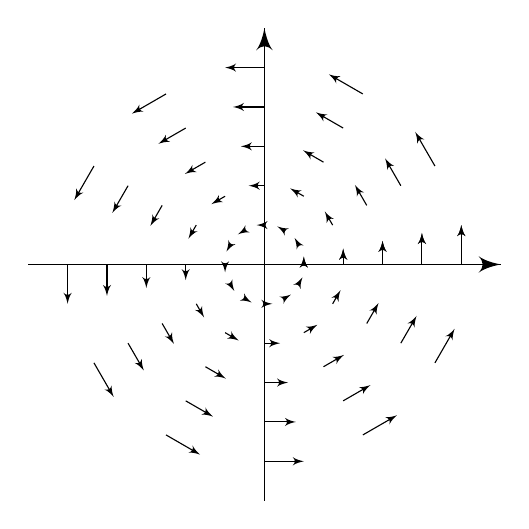
\begin{tikzpicture}
      \draw [->] (-3, 0) -- (3, 0);
      \draw [->] (0, -3) -- (0, 3);

      \foreach \t in {0,30,60,90,120,150,180,210,240,270,300,330,360} {
        \begin{scope}[rotate=\t]
          \draw [-latex'] (2.5, 0) -- +(0, 0.5);
          \draw [-latex'] (2, 0) -- +(0, 0.4);
          \draw [-latex'] (1.5, 0) -- +(0, 0.3);
          \draw [-latex'] (1, 0) -- +(0, 0.2);
          \draw [-latex'] (0.5, 0) -- +(0, 0.1);
        \end{scope}
      }
    \end{tikzpicture}
  \end{center}
  We would expect the integral curves to be circles. Indeed, suppose $\gamma: I \to \R^2$ is an integral curve. Write $\gamma = (\gamma_1, \gamma_2)$. Then we have
  \[
    \gamma_1'(t) \frac{\partial}{\partial x} + \gamma_2'(t) \frac{\partial}{\partial y} = \gamma_1(t) \frac{\partial}{\partial y} - \gamma_2(t) \frac{\partial}{\partial x}.
  \]
  So the equation is
  \begin{align*}
    \gamma_1'(t) &= \gamma_2(t)\\
    \gamma2'(t) &= \gamma_1(t).
  \end{align*}
  For example, if our starting point is $p = (1, 0)$, then we have
  \[
    \gamma_1(t) = \cos t,\quad \gamma_2(t) = \sin t.
  \]
\end{eg}
We see that to find an integral curve, all we are doing is just solving ordinary differential equations. We know that all ODE's have smooth and unique solutions, and they have all the nice properties we can hope for. So we are going to get nice corresponding results for integral solutions.

\begin{eg}
  Take $M = \R$, and
  \[
    X = x^2 \frac{\d}{\d x}.
  \]
  Then if $\gamma$ is an integral curve, then
  \[
    \gamma'(t) = \gamma(t)^2.
  \]
  This means that the solution is of the form
  \[
    \gamma(t) = \frac{1}{C - t}
  \]
  for $C$ a constant. For example, if we want $\gamma(0) = \frac{1}{2}$, then we have
  \[
    \gamma(t) = \frac{1}{2 - t}.
  \]
  The solution to this ODE is defined only for $t < 2$, so we have $I = (-\infty, 2)$.
\end{eg}

\begin{ex}
  If $\gamma: I \to M$ is an integral curve for $X \in \Vect(M)$, and $t_0 \in I$, then the map $\tilde{\gamma}: \tilde{I} \to M$ given by
  \[
    \tilde{\gamma}(t) = \gamma(t - t_0)
  \]
  is also an integral curve, where
  \[
    \tilde{I} = \{t: t - t_0 \in I\}.
  \]
\end{ex}

We are going to prove that integral curves always exist. To do so, we need to borrow some powerful theorems from ODE theory:
\begin{thm}[Fundamental theorem on ODEs]
  Let $U \subseteq \R^n$ be open and $\alpha: u \to \R^n$ smooth. Pick $t_0 \in \R$.

  Consider the ODE
  \begin{align*}
    \dot{\gamma}_i(t) &= \alpha_i(\gamma(t))\\
    \gamma_i(t_0) &= c_i,
  \end{align*}
  where $\mathbf{c} = (c_1, \cdots, c_n) \in \R^n$.

  Then there exists an open interval $I$ containing $t_0$ and an open $U_0 \subseteq U$ such that for every $\mathbf{c} \in U_0$, there is a smooth solution $\gamma_\mathbf{c}:I \to U$ satisfying the ODE.

  Moreover, any two solutions agree on a common domain, and the function $\Q: I \times U_0 \to U$ defined by $\Theta(t, \mathbf{c}) = \gamma_\mathbf{c}(t)$ is smooth (in both variables).
\end{thm}

\begin{thm}[Existence of integral curves]
  Let $X \in \Vect(M)$ and $p \in M$. Then there exists some open interval $I \subseteq \R$ with $0 \in I$ and an integral curve $\gamma: I \to M$ for $X$ with $\gamma(0) = p$.

  Moreover, if $\tilde{\gamma}: \tilde{I} \to M$ is another integral curve for $X$, and $\tilde{\gamma}(0) = p$, then $\tilde{\gamma} = \gamma$ on $I \cap \tilde{I}$.
\end{thm}

\begin{proof}
  Pick local coordinates for $M$ centered at $p$ in an open neighbourhood $U$. So locally we write
  \[
    X = \sum \alpha_i \frac{\partial}{\partial x_i},
  \]
  where $\alpha_i \in C^\infty(U)$. We want to find $\gamma = (\gamma_1, \cdots, \gamma_n): I \to U$ such that
  \[
    \sum_i \gamma_i'(t) \left.\frac{\partial}{\partial x_i}\right|_{\gamma(t)} = \sum_i \alpha_i(\gamma(t)) \left.\frac{\partial}{\partial x_i}\right|_{\gamma(t)},\quad \gamma_i(0) = 0.
  \]
  Since the $\frac{\partial}{\partial x_i}$ for a basis, this is equivalent to saying
  \[
    \gamma_i(t) = \alpha_i(\gamma(t)),\quad \gamma_i(0) = 0
  \]
  for all $i$ and $t \in I$.

  By the general theory of ordinary differential equations, there is an interval $I$ and a solution $\gamma$, and any two solutions agree on their common domain.

  However, we need to do a bit more for uniqueness, since all we know is that there is a unique integral curve lying in this particular chart. It might be that there are integral curves that do wild things when they leave the chart.

  So suppose $\gamma: I \to M$ and $\tilde{\gamma}: \tilde{I} \to M$ are both integral curves passing through the same point, ie. $\gamma(0) = \tilde{\gamma}(0) = p$.

  We let
  \[
    J = \{t \in I \cap \tilde{I}: \gamma(t) = \tilde{\gamma}(t)\}.
  \]
  This is non-empty since $0 \in J$, and $J$ is closed since $\gamma$ and $\tilde{\gamma}$ are continuous. To show it is all of $I \cap \tilde{I}$, we only have to show it is open, since $I \cap \tilde{I}$ is connected.

  So let $t_0 \in J$, and consider $q = \gamma(t_0)$. Then $\gamma$ and $\tilde{\gamma}$ are integral curves of $X$ passing through $q$. So by the first part, they agree on some neighbourhood of $t_0$. So $J$ is open. So done.
\end{proof}

\begin{defi}[Maximal integral curve]\index{maximal integral curve}\index{integral curve!maximal}
  Let $p \in M$, and $X \in \Vect(M)$. Let $I_p$ be the union of all $I$ such that there is an integral curve $\gamma: I \to M$ with $\gamma(0) = p$. Then there exists a unique integral curve $\gamma: I_p \to M$, known as the \emph{maximal integral curve}.
\end{defi}

Note that $I_p$ does depend on the point.

\begin{eg}
  Consider the vector field
  \[
    X = \frac{\partial}{\partial x}
  \]
  on $\R^2 \setminus \{0\}$. Then for any point $p = (x, y)$, if $y \not= 0$, then then $I_p = \R$, but if $y = 0$ and $x < 0$, then $I_p = (-\infty, -x)$.
  \begin{center}
    \begin{tikzpicture}
      \draw (-3, 3) rectangle (3, -3);
      \foreach \x in {-2.7, -1.7, -0.7, 0.3, 1.3, 2.3} {
         \foreach \y in {-2, -1, 0, 1, 2} {
           \draw [-latex'] (\x, \y) -- +(0.4, 0);
         }
      }
      \draw circle [radius=0.1];
    \end{tikzpicture}
  \end{center}
\end{eg}

For now, we assume $X$ is such that $I_p = \R$ for all $p \in M$. Such a vector field is said to be \emph{complete}\index{complete vector field}.

Consider $\Theta_t(p) = \gamma_p(t)$\index{$\Theta_t(p)$}, where $\gamma_p$ is the maximal integral curve of $X$ through $p$, and $\gamma(0) = p$. So $\Theta_t(p)$ is defined for all $p \in M$ and $t \in \R$. Observe that
\begin{enumerate}
  \item $\Theta_0(p) = \gamma_p(0) = p$ for all $p$.
  \item Fix $s \in \R$ and $p \in M$, and consider the map $\sigma(t) = \gamma_p(s + t)$ for all $t \in \R$. Then
    \begin{enumerate}
      \item $\sigma(0) = \gamma_p(s)$
      \item $\sigma$ is an integral curve of $X$.
    \end{enumerate}
    In other words, we have $\sigma(t) = \gamma_{\gamma_p(s)}(t)$.

    In a better notation, we have
    \[
      \Theta_t(\Theta_s(p)) = \Theta_t(\gamma_p(s)) = \sigma(t) = \Theta_{s + t}(p).
    \]
\end{enumerate}

Said another way, we have
\[
  \Theta_0 = \id,\quad \Theta_t \circ \Theta_s = \Theta_{s + t},
\]
with $\Theta_t: M \to M$.

It is a fact that $\Theta(t)$ is smooth as a map $M \to M$. So for each $t$, we have $\Theta_t \in C^\infty(M, M)$. Moreover we have
\[
  \Theta_{t} \circ \Theta_{-t} = \Theta_0 = \id,
\]
and similarly the other way round. So we have
\[
  \Theta_t^{-1} = \Theta_{-t},
\]
and in particular it is invertible.

More algebraically, if we write $\Diff(m)$ for the diffeomorphisms $M \to M$, then
\begin{align*}
  \R &\to \Diff(M)\\
  t &\mapsto \Theta_t
\end{align*}
is a homomorphism of groups. We call this a \emph{one-parameter subgroup} of diffeomorphisms.

What happens when we relax the completeness assumption? Everything is essentially the same whenever things are defined, but we have to take care of the domains of definition.

\begin{thm}
  Let $M$ be a manifold, and $X \in \Vect(M)$. Define
  \[
    D = \{(t, p) \in \R \times M: t \in I_p\}.
  \]
  In other words, this is the set of all $(t, p)$ such that $\gamma_p(t)$ exists. We set
  \[
    \Theta_t (p) = \Theta(t, p) = \gamma_p(T)
  \]
  for all $(t, p) \in D$. Then
  \begin{enumerate}
    \item $D$ is open and $\Theta: D \to M$ is smooth
    \item $\Theta(0, p) = p$ for all $p \in M$.
    \item If $(t, p) \in D$ and $(t, \Theta(s, p)) \in D$, then $(s + t, p) \in D$ and $\Theta(t, \Theta(s, p)) = \Theta(t + s, p)$.
    \item For any $t \in \R$, the set $M_t: \{p \in M: (t, p) \in D\}$ is open in $M$, and
      \[
        \Theta_t: M_t \to M_{-t}
      \]
      is a diffeomorphism with inverse $\Theta_{-t}$.
  \end{enumerate}
\end{thm}

\begin{proof}
  Exercise.
\end{proof}

This is really annoying. We now prove the following useful result that saves us from worrying about these problems in nice cases:
\begin{prop}
  Let $M$ be a compact manifold. Then any $X \in \Vect(M)$ is complete.
\end{prop}

\begin{proof}
  Recall that
  \[
    D = \{(t, p): \Theta_t(p)\text{ is defined }\}
  \]
  is open. So given $p \in M$, there is some open neighbourhood $U \subseteq M$ of $p$ and an $\varepsilon > 0$ such that $(-\varepsilon, \varepsilon) \times U \subseteq D$. By compactness, we can find finitely many such $U$ that cover $M$, and find a small $\varepsilon$ such that $(-\varepsilon, \varepsilon) \times M \subseteq D$.

  In other words, we know $\Theta_t(p)$ exists and $p \in M$ and $|t| < \varepsilon$. Also, we know $\Theta_t \circ \Theta_s = \Theta_{t + s}$ whenever $|t|, |s| < \varepsilon$, and in particular $\Theta_{t + s}$ is defined. So $\Theta_{Nt} = (\Theta_t)^N$ is defined for all $N$ and $|t| < \varepsilon$, so $\Theta_t$ is defined for all $t$.
\end{proof}

\subsection{Lie derivative}
Let $X \in \Vect(M)$ be a complete vector field with flow $\Theta$. We want to use $\Theta$ to differentiate ``essentially anything'' in the direction of $X$.

\begin{notation}\index{$F^*g$}
Let $F: M \to M$ be a diffeomorphism, with $g \in C^\infty(M, \R)$. We write
\[
  F^* g = g \circ F \in C^\infty(M, \R).
\]
\end{notation}

For each $t \in \R$, we have a diffeomorphism $\Theta_t: M \to M$.
\begin{defi}[Lie derivative of function]\index{Lie derivative!function}
  Let $X$ be a complete vector field, and $\Theta$ be its flow. We define the \emph{Lie derivative} of $g$ along $X$ by
  \[
    \mathcal{L}_X(g) = \left.\frac{\d}{\d t} \right|_{t = 0} \Theta_t^* g.
  \]
  Here this is defined pointwise, ie. for all $p \in M$, we define
  \[
    \mathcal{L}_X(g)(p) = \left.\frac{\d}{\d t}\right| \Theta_t^*(g)(p).
  \]
\end{defi}

\begin{lemma}
  $\mathcal{L}_X(g) = X(g)$. In particular, $\mathcal{L}_X(g) \in C^\infty(M, \R)$.
\end{lemma}

\begin{proof}
  \[
    \mathcal{L}_X(g)(p) = \left.\frac{\d}{\d t}\right| \Theta_t^*(g)(p) = \left.\frac{\d}{\d t}\right|_{t = 0} g(\Theta_t(p)) = X(p).
  \]
\end{proof}

So this is quite boring. However, we can do something more exciting by differentiating vector fields.

\begin{notation}\index{$F^*(Y)$}
  Let $Y \in \Vect(M)$, and $F: M \to M$ be a diffeomorphism. Then $\D F^{-1}|_{F(p)}: T_{F(p)} M \to T_pM$. So we can write
  \[
    F^*(Y)|_p = \D F^{-1}|_{F(p)}(Y_{F(p)}) \in T_p M.
  \]
  Then $F^*(Y) \in \Vect(M)$. If $g \in C^\infty(M)$, then
  \[
    F^*(Y)|_p(g) = Y_{F(p)} (g \circ F^{-1}).
  \]
  Alternatively, we have
  \[
    F^*(Y)|_p(g \circ F) = Y_{F(p)}(g).
  \]
  Removing the $p$'s, we have
  \[
    F^*(Y)(g \circ F) = (Y(g)) \circ F.
  \]
\end{notation}

\begin{defi}[Lie derivative of vector field]\index{Lie derivative!vector field}
  Let $X \in \Vect(M)$ be complete, and $Y \in \Vect(M)$ be a vector field. Then the \emph{Lie derivative} is given pointwise by
  \[
    \mathcal{L}_X(Y) = \left.\frac{\d}{\d t}\right|_{t = 0} \Theta_t^*(Y).
  \]
\end{defi}

\begin{lemma}
  We have
  \[
    \mathcal{L}_X Y = [X, Y].
  \]
\end{lemma}

\begin{proof}
  Let $g \in C^\infty(M, \R)$. Then we have
  \[
    \Theta_t^*(Y)(g \circ \Theta_t) = Y(g) \circ \Theta_t.
  \]
  We now look at
  \[
    \frac{\Theta_t^* (Y)(g) - Y(g)}{t} = \underbrace{\frac{\Theta_t^*(Y)(g) - \Theta_t^*(Y)(g \circ \Theta_t)}{t}}_{\alpha_t} + \underbrace{\frac{Y(g) \circ \Theta_t - Y(g)}{t}}_{\beta_t}.
  \]
  We have
  \[
    \lim_{t \to 0} \beta_t = \mathcal{L}_X (Y(g)) = XY(g)
  \]
  by the previous lemma, and we have
  \[
    \lim_{t\to 0}\alpha_t = \lim_{t \to 0} (\Theta_t^*(Y))\left(\frac{g - g \circ \Theta_t}{t}\right) = Y(-L_X(g)) = - YX(g).
  \]
\end{proof}

\begin{cor}
  Let $(X, Y) \in \Vect(M)$ and $f \in C^\infty(M, \R)$. Then
  \begin{enumerate}
    \item $\mathcal{L}_X(fY) = \mathcal{L}_X(f) Y + f \mathcal{L}_X Y = X(f) Y + f \mathcal{L}_X Y$
    \item $\mathcal{L}_X Y = - \mathcal{L}_Y X$
    \item $\mathcal{L}_X[Y, Z] = [\mathcal{L}_X Y, Z] + [Y, \mathcal{L}_X Z]$.
  \end{enumerate}
\end{cor}

\begin{proof}
  Immediate from the properties of the Lie bracket.
\end{proof}

\section{Lie groups}
\begin{defi}[Lie group]\index{Lie group}
  A \emph{Lie group} is a manifold $G$ with a group structure such that multiplication $m: G \times G \times G$ and inverse $i: G \to G$ are smooth maps.
\end{defi}

\begin{own}
  \begin{defi}[Lie group]
    A \emph{Lie group} is a group object in the category of smooth manifolds.
  \end{defi}
\end{own}

\begin{eg}
  $\GL_n(\R)$ and $\GL_n(\C)$ are Lie groups.
\end{eg}

\begin{eg}
  $M_n(R)$ under addition is also a Lie group.
\end{eg}

\begin{eg}
  $\Or(n)$ is a Lie group.
\end{eg}

\begin{notation}\index{$L_g$}
  Let $G$ be a Lie group and $g \in G$. We write $L_g: G \to G$ for the diffeomorphism.
  \[
    L_g(h) = gh.
  \]
\end{notation}
The thing about Lie groups is that they have an enormous amount of symmetry. Given any local information near an element $g$, we can transfer it to local information near $h$ by applying the diffeomorphism $L_{hg^{-1}}$.

So in particular, knowing how the Lie group behaves locally (or even infinitesimally) near the identity tells us a lot about the Lie group. In particular, the diffeomorphism $L_g; G \to G$ induces a linear isomorphism $\D L_g|_e : T_e G \to T_g G$.

\begin{defi}[Left invariant vector field]\index{left invariant vector field}\index{vector field!left invariant}
  Let $X \in \Vect(G)$ be a vector field. This is \emph{left invariant} if
  \[
    \D L_g|_h (X_h) = X_{gh}
  \]
  for all $h \in G$.
\end{defi}

Let $\Vect^L(G)$ be the collection of all left invariant vector field. If $X, Y \in \Vect^L(G)$, then so is $[X, Y]$. So $\Vect^L(G)$ is a Lie subalgebra of $\Vect(G)$.

\begin{lemma}
  Given $\zeta \in T_e G$, we let $X_\zeta(g) = \D L_g(\zeta) \in T_g(G)$. Then the map $T_e G \to \Vect^L(G)$ by $X \mapsto X_\zeta$ is an isomorphism of vector spaces.
\end{lemma}

\begin{proof}
  The inverse is given by $X \mapsto X|_e$. The only thing to check is that $X_\zeta$ actually is a left invariant vector field. The left invariant part follows from
  \[
    \D L|_h (X_\zeta|_g) = \D L_h \D L_g (\zeta) = \D L_{hg}(\zeta) = X_\zeta |_{hg}.
  \]
  To check that $X_\zeta$ is smooth, suppose $f \in C^\infty(U, \R)$, where $U$ is open and contains $e$. We let $\gamma: (-\varepsilon, \varepsilon) \to U$ be smooth with $\dot{\gamma}(0) = \zeta$. So
  \[
    X_\zeta f|_g = \D L_g (\zeta)(f) = \zeta(f \circ L_g) = \left.\frac{\d}{\d t}\right|_{t = 0} (f \circ L_g \circ \gamma)
  \]
  But as $(t, g) \mapsto f \circ L_g \circ \gamma(t)$ is smooth, it follows that $X_\zeta f$ is smooth. So $X_\zeta \in \Vect^L(G)$.
\end{proof}

\begin{defi}[Lie algebra of Llie group]\index{Lie algebra of Lie group}
  let $G$ be a lie group. The \emph{Lie algebra} $\mathfrak{g}$ of $G$ is the Lie algebra $T_eG$ whose Lie bracket is induced by that of the isomorphism with $\Vect^L(G)$. So
  \[
    [\zeta, \eta] = [X_\zeta, X_\eta]|_e.
  \]
  We also write $\Lie(G)$ for $\mathfrak{g}$.
\end{defi}

Note that $\dim \mathfrak{g} = \dim G$ is finite.

\begin{eg}
  For any vector space $V$ and $v \in V$, we have $T_v V \cong V$.
\end{eg}

\begin{eg}
  In particular, if $M_{n, n}$ is the $n \times n$ matrices under addition. Then $T_A M_n \cong M_n$ if $A \in M_n$.

  Now note that $G = \GL_n(\R)$ is an open subset of $M_n$. Then
  \[
    \gl_n(\R) = \Lie(\GL_n(\R)) = T_I \GL_n = T_I M_n \cong M_n.
  \]
  If $A, B \in \GL_n$, then
  \[
    L_A(B) = AB.
  \]
  So
  \[
    \D L_A|_B(H) = AH
  \]
  as $L_A$ is linear.

  We claim that under the identification, if $\zeta, \eta \in \gl_n(\R) = M_n$, then
  \[
    [\zeta, \eta] = \zeta \eta - \eta \zeta.
  \]
  Indeed, on $G$, we have global coordinates $U_i^j: \GL_n \to \R$ where
  \[
    U_i^j(A) = A_i^j,
  \]
  where $A = (A_i^j) \in \GL_n$.

  Under this chart, we have
  \[
    X_\zeta|_A = L_A(\zeta) = \sum_{ij} (A \zeta)_j^i \left.\frac{\partial}{\partial U_j^i}\right|_A = \sum A_k^i \zeta_j^k \left.\frac{\partial}{\partial U_j^i} \right|_A
  \]
  So we have
  \[
    X_\zeta = \sum_{i,j,k} U^i_k \zeta^k_j \frac{\partial}{\partial U_j^i}.
  \]
  So we have
  \[
    [X_\zeta, X_\eta] = \left[\sum_{i,j,k} U_k^i \zeta_j^k \frac{\partial}{\partial U_j^i},\sum_{p, q, r} U_q^p \eta_r^p \frac{\partial}{\partial U_r^p}\right].
  \]
  We now use the fact that
  \[
    \frac{\partial}{\partial U^i_j} U^p_q = \delta_{ip}\delta_{jq}.
  \]
  We then expand
  \[
    [X_\zeta, X_\eta] = \sum_{i,j,k,r} (U_j^i \zeta_k^j \eta^k_r - U^i_j \zeta^j_k \zeta^k_r) \frac{\partial}{\partial U_r^i}.
  \]
  So we have
  \[
    [X_\zeta, X_\eta] = X_{\zeta\eta - \eta\zeta}.
  \]
\end{eg}

\begin{defi}[Lie group homomorphisms]\index{Lie group!homomorphism}
  Let $G, H$ be Lie groups. A \emph{Lie group homomorphism} is a smooth map that is also a homomorphism.
\end{defi}

\begin{defi}[Lie algebra homomorphism]\index{Lie algebra!homomorphism}
  Let $\mathfrak{g}, \mathfrak{h}$ be Lie group homomorphisms. Then a \emph{Lie algebra homomorphism} is a linear map $\beta: \mathfrak{g} \to \mathfrak{h}$ such that
  \[
    \beta[\zeta,\eta] = [\beta(\zeta), \beta(\eta)].
  \]
\end{defi}

\begin{prop}
  Let $G$ be a Lie group and $\zeta \in \mathfrak{g}$. Then the integral curve $\gamma$ for $X_\zeta$ through $e \in G$ exists for all time, and $\gamma: \R \to G$ is a Lie group homomorphism.
\end{prop}

The idea is that once we have a small integral curve, we can use the Lie group structure to copy the curve to patch together a long integral curve.
\begin{proof}
  Let $\gamma: I \to G$ be a maximal integral curve of $X_\zeta$, say $(-\varepsilon, \varepsilon) \in I$. We fix a $t_0$ with $|t_0| < \varepsilon$. Consider $g_0 = \gamma(t_0)$.

  We let
  \[
    \tilde{\gamma}(t) = L_{g_0}(\gamma(t))
  \]
  for $|t| < \varepsilon$.

  We claim that $\tilde{\gamma}$ is an integral curve of $X_\zeta$ with $\tilde{\gamma}(0) = g_0$. Indeed, we have
  \[
    \dot{\tilde{\gamma}}|_t = \frac{\d}{\d t} L_{g_0}\gamma(t) = \D L_{g_0} \dot{\gamma}(t) = \D L_{g_0} X_\zeta|_{\gamma(t)} = X_\zeta|_{\gamma_0 \cdot \gamma(t)} = X_\zeta|_{\tilde{\gamma}(t)}.
  \]
  By patching these together, we know $(t_0 - \varepsilon, t_0 + \varepsilon) \subseteq I$. Since we have a fixed $\varepsilon$ that works for all $t_0$, it follows that $I = \R$.

  The fact that this is a Lie group homomorphism follows from general properties of flow maps.
\end{proof}

\begin{eg}
  Let $G = \GL_n$. If $\zeta \in \gl_n$, we set
  \[
    e^\zeta = \sum_{k \geq 0} \frac{1}{k!} \zeta^k.
  \]
  We set $F(t) = e^{t \zeta}$. We observe that this is in $\GL_n$ since $e^{t\zeta}$ has an inverse $e^{-t\zeta}$ (alternatively, $\det (e^{t\zeta}) = e^{\tr (t\zeta)} \not= 0$). Then
  \[
    F'(t) = \frac{\d}{\d t} \sum_k \frac{1}{k!} t^k \zeta^k = e^{t\zeta} \zeta = L_{e^{t\zeta}}\zeta = L_{F(t)}\zeta.
  \]
  Also, $F(0) = I$. So $F(t)$ is an integral curve.
\end{eg}

\begin{defi}[Exponential map]\index{exponential map}
  The \emph{exponential map} of a Lie group $G$ is $\exp: \mathfrak{g} \to G$ given by
  \[
    \exp(\zeta) = \gamma_\zeta(1),
  \]
  where $\zeta$ is the integral curve of $X_\zeta$ through $e \in G$.
\end{defi}
So in the case of $G = \GL_n$, the exponential map is the exponential map.

\begin{prop}\leavevmode
  \begin{enumerate}
    \item $\exp$ is a smooth map.
    \item If $F(t) = \exp(t\zeta)$, then $F: \R \to G$ is a Lie group homomorphism and $\D F|_0 \left(\frac{\d}{\d t}\right) = \zeta$.
    \item The derivative
      \[
        \D \exp: T_0 \mathfrak{g} \cong \mathfrak{g} \to T_e G \cong \mathfrak{g}
      \]
      is the identity map.
    \item $\exp$ is a local diffeomorphism around $0 \in \mathfrak{g}$, ie. there exists an open $U \subseteq \mathfrak{g}$ containing $0$ such that $\exp: U \to \exp(U)$ is a diffeomorphism.
    \item $\exp$ is natural, ie. if $f: G \to H$ is a Lie group homomorphism, then the diagram
      \[
        \begin{tikzcd}
          \mathfrak{g} \ar[r, "\exp"] \ar[d, "\D f|_e"]& G \ar[d, "f"]\\
          \mathfrak{h} \ar[r, "\exp"] & H
        \end{tikzcd}
      \]
      commutes.
  \end{enumerate}
\end{prop}

\begin{proof}\leavevmode
  \begin{enumerate}
    \item This is the smoothness of ODE's with respect to parameters
    \item Exercise.
    \item If $\zeta \in \mathfrak{g}$, we let $\sigma(t) = t \zeta$. So $\dot{\sigma}(0) = \zeta \in T_0 \mathfrak{g} \cong \mathfrak{g}$. So
      \[
        \D \exp|_0 (\zeta) = \D \exp|_0(\dot{\sigma}(0)) = \left.\frac{\d}{\d t}\right|_{t = 0} \exp(\sigma(t)) = \left.\frac{\d}{\d t}\right|_{t = 0} \exp(t \zeta) = X_\zeta|_e = \zeta.
      \]
    \item Follows from above by inverse function theorem.
    \item Exercise.
  \end{enumerate}
\end{proof}

\begin{defi}[Lie subgroup]\index{Lie subgroup}\index{Lie group!subgroup}
  A \emph{Lie subgroup} of $G$ is a subgroup $H$ with a smooth structure on $H$ making $H$ an \emph{immersed} submanifold.
\end{defi}

Certainly, if $H \subseteq G$ is a Lie subgroup, then $\mathfrak{h} \subseteq \mathfrak{g}$ is a Lie subalgebra.

\begin{thm}
  If $\mathfrak{h} \subseteq \mathfrak{g}$ is a subalgebra, then there exists a unique connected Lie subgroup $H \subseteq G$ such that $\Lie(H) = \mathfrak{h}$.
\end{thm}

\section{Tensors}
We are going to do linear algebra! In all of maths, we eventually get to the point where we simplified everything and took linear approximations, and then we have to do linear algebra. So let's learn linear algebra.

We are going to talk about things like bilinear maps. A bilinear maps is a function that takes in two vectors and returns a number, and this is linear in both variables. An example is the inner product, and another example is the volume form, which tells us the volume of a parallelopiped spanned by the two vectors.

\begin{defi}[Bilinear map]\index{bilinear map}
  Let $U, V, W$ be vector spaces. We define $\Bilin(V\times W, U)$ to be the functions $V \times W \to U$ that are bilinear, ie.
  \begin{align*}
    \alpha(\lambda_1 v_1 + \lambda_2 v_2, w) &= \lambda_1 \alpha(v_1, w) + \lambda_2 \alpha(v_2, w)\\
    \alpha(v, \lambda_1 w_1 + \lambda_2 w_2) &= \lambda_1 \alpha(v, w_1) + \lambda_2 \alpha(v, w_2).
  \end{align*}
\end{defi}
It is important that a bilinear map is not a linear map. This is bad. We spent so much time studying linear maps, and we now have to go back to our linear algebra book and rewrite everything to talk about bilinear maps as well. But bilinear maps are not enough. We want to do them for multi-linear maps! Linear maps were already complicated enough, and we now have many other dimensions to talk about. We want to die.

Tensors are a trick to turn the study of bilinear maps to linear maps (from a different space).

\begin{defi}[Tensor product]\index{tensor product}
  A \emph{tensor product} of two vector spaces $V, W$ is a vector space $V \otimes W$ and a bilinear map $\pi: V \times W \to V \otimes W$ such that a bilinear map from $V \times W$ is ``the same as'' a linear map from $V \times W$. More precisely, given any bilinear map $\alpha: V \times W \to U$, we can find a unique linear map $\tilde{\alpha}: V \otimes W \to U$ such that the following diagram commutes:
  \[
    \begin{tikzcd}
      V \times W \ar[rd, "\alpha"] \ar[d, "\pi"] \\
      V \otimes W \ar[r, "\tilde\alpha"'] & U
    \end{tikzcd}
  \]
  So we have
  \[
    \Bilin(V \times W, U) \cong \Hom(V \otimes W, U).
  \]
  Given $v \in V$ and $w \in W$, we obtain $\pi(v, w) \in V \otimes W$, called the \emph{tensor product} of $v$ and $w$, written $v \otimes w$.
\end{defi}
We say $V \otimes W$ \emph{represents} bilinear maps from $V \times W$.

It is important to note that not all elements of $V \otimes W$ are of the form $v \otimes w$.

\begin{prop}
  Given maps $f: V \to W$ and $g: V' \to W'$, then we obtain a map $f \otimes g: V \otimes V' \to W \otimes W'$ given by the bilinear map
  \[
    (f \otimes g)(v, w) = f(v) \otimes g(w).
  \]
\end{prop}

\begin{lemma}
  Tensor products exist (and are unique up to isomorphism) for all pairs of vector spaces.
\end{lemma}

\begin{proof}
  Exercise
\end{proof}

\begin{lemma}
  Given $v, v_i \in V$ and $w, w_i \in V$ and $\lambda_i \in \F$, we have
  \begin{align*}
    (\lambda_1 v_1 + \lambda_2 v_2) \otimes w &= \lambda_1 (v_1 \otimes w) + \lambda_2 (v_2 \otimes w)\\
    v \otimes (\lambda_1 w_1 + \lambda_2 w_2) &= \lambda_1 (v \otimes w_1) + \lambda_2 (v \otimes w_2).
  \end{align*}
\end{lemma}

\begin{proof}
  Immediate from definition of bilinear map.
\end{proof}

\begin{lemma}
  If $v_1,\cdots, v_n$ is a basis of $V_1$, and $w_1, \cdots, w_m$ are a basis for $W$, then
  \[
    \{v_i \otimes w_j: i = 1, \cdots, n; j = 1, \cdots, m\}
  \]
  is a basis for $V \otimes W$. In particular, $\dim V \otimes W = \dim V \times \dim W$.
\end{lemma}

\begin{proof}
  We have $V \otimes W = \Bilin(V \times W, \R)^*$. We let $\alpha_{pq}:V \times W \to \R$ be given by
  \[
    \alpha_{pq}\left(\sum a_i v_i, \sum b_j w_j\right) = a_p b_q.
  \]
  Then $\alpha_{pq} \in \Bilin(V\times W, \R)$, and $(v_i \otimes w_j)$ are dual to $\alpha_{pq}$. So it suffices to show that $\alpha_{pq}$ are a basis. It is clear that they are independent, and any bilinear map can be written as
  \[
    \alpha = \sum c_{pq}\alpha_{pq},
  \]
  where
  \[
    c_{pq} = \alpha(v_p, w_q).
  \]
  So done.
\end{proof}

\begin{prop}
  For any vector spaces $V, W, U$, we have (natural) isomorphisms
  \begin{enumerate}
    \item $V \otimes W \cong W \otimes W$
    \item $(V \otimes W) \otimes U \cong V \otimes (W \otimes U)$
    \item $(V \otimes W)^* \cong V^* \otimes W^*$
  \end{enumerate}
\end{prop}

\begin{defi}[Covariant tensor]\index{covariant tensor}
  A \emph{covariant tensor} of rank $k$ on $V$ is an element of
  \[
    \alpha \in \underbrace{V^* \otimes \cdots \otimes V^*}_{k\text{ times}},
  \]
  ie. $\alpha$ is a multilinear map $V \times \cdots \times V \to \R$.
\end{defi}

\begin{eg}
  A covariant $1$-tensor is an $\alpha \in V^*$, ie. a linear map $\alpha: V \to \R$.

  A covariant $2$-tensor is a $\beta \in V^* \otimes V^*$, ie. a bilinear map $V \times V \to \R$, eg. an inner product.
\end{eg}

\begin{eg}
  If $\alpha, \beta \in V^*$, then $\alpha \otimes \beta \in V^* \otimes V^*$ is the covariant $2$-tensor given by
  \[
    (\alpha \otimes b)(v, w) = \alpha(v) \beta(w).
  \]
  More generally, if $\alpha$ is a rank $k$ tensor and $\beta$ is a rank $\ell$ tensor, then $\alpha \otimes \beta$ is a rank $k + \ell$ tensor.
\end{eg}

\begin{defi}[Tensor]\index{tensor}
  A \emph{tensor} of type $(k, \ell)$ is an element in
  \[
    T^k_\ell(V) = \underbrace{V^* \otimes \cdots \otimes V^*}_{k\text{ times}} \otimes \underbrace{V \otimes \cdots \otimes V}_{\ell\text{ times}}.
  \]
\end{defi}
We are interested in alternating bilinear maps, ie. $\alpha(v, w) = - \alpha(w, v)$, or equivalently, $\alpha(v, v) = 0$ (if the characteristic is not $2$).

\begin{defi}[Exterior product]\index{exterior product}\index{exterior algebra}.
  Consider
  \[
    T(V) = \otimes_{k \geq 0} V^{\otimes k}
  \]
  as an algebra (with multiplication given by the tensor product) (with $V^{\otimes 0} = \R$). We let $I(V)$ be the ideal (as algebras!) generated by $\{v \otimes v: v \in V\} \subseteq T(V)$. We define
  \[
    \Lambda V = T(V)/I(V),
  \]
  with a projection map $\pi: T(V) \to \Lambda(V)$. This is known as the \emph{exterior algebra}. We let
  \[
    \Lambda^k(V) = \pi(V^{\otimes k}),
  \]
  the \emph{$k$-th exterior product} of $V$.

  We write $a \wedge b$ for $\pi(\alpha \otimes \beta)$.
\end{defi}

The idea is that $\Lambda^p V$ is the dual of the space of alternating multilinear maps $V \times V\to \R$.

\begin{lemma}\leavevmode
  \begin{enumerate}
    \item If $\alpha \in \Lambda^p V$ and $\beta \in \Lambda^q V$, then $\alpha \wedge \beta = (-1)^{pq} \beta \wedge \alpha$.
    \item If $\dim V = n$, then we have
      \[
        \dim \Lambda^0 V = 1,\quad \dim \Lambda^n V = 1,\quad \Lambda^p V = \{0\}.
      \]
    \item The multilinear map $\det: V \times \cdots \times V \to \R$ spans $\Lambda^n V$.
    \item If $v_1, \cdots, v_n$ is a basis for $V$, then
      \[
        \{v_{i_1} \wedge \cdots \wedge v_{i_p}: i_1 < \cdots < i_p\}
      \]
      is a basis for $\Lambda^p v$.
  \end{enumerate}
\end{lemma}

\begin{proof}\leavevmode
  \begin{enumerate}
    \item We clearly have $v \wedge v = 0$. So
      \[
        v \wedge w = - w \wedge v
      \]
      Then
      \[
        (v_1 \wedge \cdots \wedge v_p) \wedge (w_1 \wedge \cdots \wedge w_q) = (-1)^{pq} w_1 \wedge \cdots \wedge w_q \wedge v_1 \wedge \cdots \wedge v_p
      \]
      since we have $pq$ swaps. Since
      \[
        \{v_{i_1} \wedge \cdots \wedge v_{i_n}: i_1, \cdots, i_p \in \{1,\cdots, n\}\} \subseteq \Lambda^p V
      \]
      spans $\Lambda^p V$ (by the corresponding result for tensor products), the result follows from linearity.
    \item Exercise.
    \item The $\det$ map is non-zero. So it follows from the above.
    \item We know that
      \[
        \{v_{i_1} \wedge \cdots \wedge v_{i_n}: i_1, \cdots, i_p \in \{1,\cdots, n\}\} \subseteq \Lambda^p V
      \]
      spans, but they are not independent since there is a lot of redundancy (eg. $v_1 \wedge v_2 = - v_2 \wedge v_1$). By requiring $i_1 < \cdots < i_p$, then we obtain a unique copy for combination.

      To check independence, we write $I = (v_{i_1}, \cdots, v_{i_p})$ and let $v_I = v_{i_1} \wedge \cdots \wedge v_{i_p}$. Then suppose
      \[
        \sum_I a_I v_I = 0
      \]
      for $a_i \in R$. For each $I$, we let $J$ be the multi-index $J = \{1, \cdots, n\} \setminus I$. So if $I \not= I'$, then $v_{I'} \wedge v_J = 0$. So wedging with $v_J$ gives
      \[
        \sum_{I'} \alpha_{I'} v_{I'} \wedge v_J = a_I v_I \wedge v_J = 0.
      \]
      So $a_I = 0$. So done by (ii).
  \end{enumerate}
\end{proof}

If $F: V \to W$ is a linear map, then we get an induced linear map $\Lambda^p F: \Lambda^p V \to \Lambda^p W$ in the obvious way, making the following diagram commute:
\[
  \begin{tikzcd}
    V^{\otimes k} \ar[r, "F^{\otimes k}"] \ar[d] & W^{\otimes k}\ar[d]\\
    \Lambda^p V \ar[r, "\Lambda^p F"] & \Lambda^p W
  \end{tikzcd}
\]
More concretely, we have
\[
  \Lambda^p F (v_1 \wedge \cdots \wedge v_p) = F(v_1) \wedge \cdots \wedge F(v_p).
\]
\begin{lemma}
  Let $F: V \to V$ be a linear map. Then $\Lambda^n F: \Lambda^n V \to \Lambda^n V$ is multiplication by $\det F$.
\end{lemma}

\begin{proof}
  Let $v_1, \cdots, v_n$ be a basis. Then $\Lambda^n V$ is spanned by $v_1 \wedge \cdots \wedge v_n$ So we have
  \[
    (\Lambda^n F)(v_1\wedge \cdots \wedge v_n) = \lambda v_1 \wedge \cdots \wedge v_n
  \]
  for some $\lambda$. Write
  \[
    F(v_i) = \sum_j A_{ji} v_j
  \]
  for some $A_{ji} \in \R$, ie. $A$ is the matrix representation of $F$. Then we have
  \[
    (\Lambda^n F)(v_1 \wedge \cdots \wedge v_n) \left(\sum_j A_j v_j\right) \wedge \cdots \wedge \left(\sum_j A_{ji} v_j\right).
  \]
  If we expand the thing in the right, a lot of things die. The only things that live are those where we get each of $v_i$ once in the wedges in some order. Then this becomes
  \[
    \sum_{\sigma \in S_n} \varepsilon(\sigma) (A_{\sigma(1), 1} \cdots A_{\sigma(n), n}) v_1 \wedge \cdots \wedge v_n = \det(F) v_1 \wedge \cdots \wedge v_n,
  \]
  where $\varepsilon(\sigma)$ is the sign of the permutation, which comes from rearranging the $v_i$ to the right order.
\end{proof}

\section{Vector bundles}
Our aim is to consider spaces $T_p M \otimes T_p M, \ldots, \Lambda^p T_p M$ etc as $p$ varies. We want to understand what it means for these vector spaces to vary smoothly with respect to $p$.

As before, our strategy is to take the union of all of them, and put some smooth structure on them.

To do so, we come up with the general notion of a vector bundle.
\begin{defi}[Vector bundle]\index{vector bundle}
  A \emph{vector bundle} of rank $r$ on $M$ is a smooth manifold $E$ with a smooth $\pi: E \to M$ such that
  \begin{enumerate}
    \item For each $p \in M$, the fibre $\pi^{-1}(p) = E_p$ is an $r$-dimensional vector space,
    \item For all $p \in M$, there is an open $U \subseteq M$ containing $p$ and a diffeomorphism
      \[
        t: E_U = \pi^{-1}(U) \to U \times \R^r
      \]
      such that
      \[
        \begin{tikzcd}
          E_U \ar[r, "t"] \ar[d, "\pi"] & U \times \R^r \ar[dl, "p_1"]\\
          U
        \end{tikzcd}
      \]
      commutes, and the induced maps $E_q \to \{q\} \times \R^r$ is a linear isomorphism for all $q \in U$.

      We call $t$ a \term{trivialization} of $E$ over $U$; call $E$ the \term{total space}; call $M$ the \term{base space}; and call $\pi$ the \term{projection}. Also, for each $q \in M$, the vector space $E_q = \pi^{-1}(\{q\})$ is called the \term{fiber} over $q$.
  \end{enumerate}
  Note that the vector space structure on $E_p$ is part of the data of a vector bundle.
\end{defi}

Alternatively, $t$ can be given by collections of smooth maps $s_1, \cdots, s_r: U \to E$ with the property that for each $q \in U$, the vectors $s_1(q), \cdots, s_r(q)$ is a basis for $E_q$. Indeed, given such $s_1, \cdots, s_r$, we can define $t$ by
\[
  t(v_q) = (q, \alpha_1, \cdots, \alpha_n),
\]
where $v_q \in E_q$ and the $\alpha_i$ are chosen such that
\[
  v_q = \sum_{i = 1}^r \alpha_i s_i(q).
\]
The $s_1, \cdots, s_r$ are known as a \term{frame} for $E$ over $U$.

\begin{eg}[Tangent bundle]
  The bundle $TM \to M$ is a vector bundle. Given any point $p$, find some coordinate charts around $p$ with coordinates $x_1, \cdots, x_n$. Then we get a frame $\frac{\partial}{\partial x_i}$, giving trivializations of $TM$ over $U$. So $TM$ is a vector bundle.
\end{eg}

\begin{defi}[Section]\index{section}\index{$C^\infty(U, E)$}
  A \emph{(smooth) section} of a vector bundle $E \to M$ over some open $U \subseteq M$ is a smooth $s: U \to E$ such that $s(p) \in E_p$ for all $p \in U$. We write $C^\infty(U, E)$ for the set of smooth sections of $E$ over $U$.
\end{defi}

\begin{eg}
  $\Vect(M) = C^\infty (M, TM)$.
\end{eg}

\begin{defi}[Transition function]\index{transition function}
  Suppose that $t_\alpha: E|_{U_\alpha} \to U_\alpha \times \R^r$ and $t_\beta: E|_{U_\beta} \to U_\beta \times \R^r$ are trivializations of $e$. Then
  \[
    t_\alpha \circ t_\beta^{-1} : (U_\alpha \cap U_\beta) \times \R^r \to (U_\alpha \cap U_\beta) \times \R^r
  \]
  is a fiberwise linear, ie.
  \[
    t_\alpha \circ t_\beta^{-1}(q, v) = (q, \varphi_{\alpha\beta}(q) v),
  \]
  where $\varphi_{\alpha\beta}(q)$ is in $\GL(r, \R)$.

  In fact, $\varphi_{\alpha\beta}: U_\alpha \cap U_\beta \to \GL_r(\R)$ is smooth. Then $\varphi_{\alpha\beta}$ is known as the \term{transition function} from $\beta$ to $\alpha$.
\end{defi}

\begin{prop}
  We have the following equalities whenever everything is defined:
  \begin{enumerate}
    \item $\varphi_{\alpha\alpha} = \id$
    \item $\varphi_{\alpha\beta} = \varphi_{\beta\alpha}^{-1}$
    \item $\varphi_{\alpha\beta}\varphi_{\beta\gamma} = \varphi_{\alpha\gamma}$, where $\varphi_{\alpha\beta} \varphi_{\beta\gamma}$ is pointwise matrix multiplication.
  \end{enumerate}
  These are known as the \term{cocycle conditions}.
\end{prop}
We now consider general constructions that allow us to construct new vector bundles from old.

We want the converse, namely that we can construct vector bundles given transition maps with these cocycle conditions.

\begin{prop}[Vector bunlde construction]
  Suppose that for each $p \in M$, we have a vector space $E_p$. We set
  \[
    E = \bigcup_p E_p
  \]
  We let $\pi: E \to M$ be given by $\pi(v_p) = p$ for $v_p \in E_p$. Suppose there is an open cover $\{U_\alpha\}$ of open sets of $M$ such that for each $\alpha$, we have maps
  \[
    t_\alpha: E|_{U_\alpha} = \pi^{-1}(U_\alpha) \to U_\alpha \times \R^n
  \]
  over $U_\alpha$ that induce fiberwise linear isomorphisms. Suppose the transition functions $\varphi_{\alpha\beta}$ are smooth. Then there exists a unique smooth structure on $E$ making $\pi: E \to M$ a vector bundle such that the $t_\alpha$ are trivializations for $E$.
\end{prop}

\begin{proof}
  The same as the case for the tangent bundle.
\end{proof}

We let $\varphi_{\alpha\varsigma}$ be transition functions for $\{t_\alpha\}$ and $\tilde{\varphi}_{\alpha\beta}$ be transition functions for $\{\tilde{t}_\alpha\}$.

\begin{defi}[Direct sum of vector bundles]\index{direct sum!vector bundles}\index{vector bundle!direct sum}
  Let $E, \tilde{E}$ be vector bundles on $M$. Suppose $t_\alpha: E|_{U_\alpha} \cong U_\alpha \times \R^r$ is a trivialization for $E$ over $U_\alpha$, and $\tilde{t}_\alpha: E|_{U_\alpha} \cong U_\alpha \times \R^{\tilde{r}}$ is a trivialization for $E$ over $U_\alpha$.

  We let $\varphi_{\alpha\varsigma}$ be transition functions for $\{t_\alpha\}$ and $\tilde{\varphi}_{\alpha\beta}$ be transition functions for $\{\tilde{t}_\alpha\}$.

  Define
  \[
    E \oplus \tilde{E} = \bigcup_p E_p \oplus \tilde{E}_p,
  \]
  and define
  \[
    T_\alpha: (E \oplus \tilde{E})|_{U_\alpha} = E|_{U_\alpha} \otimes \tilde{E}|_{U_\alpha} \to U_\alpha \times (\R^n \oplus \R^{\tilde{r}} = U_\alpha \times \R^{r + \tilde{r}}
  \]
  be the fiberwise direct sum of the two trivializations. Then $T_\alpha$ clearly gives a linear isomorphism $(E \oplus \tilde{E})_p \cong \R^{r + \tilde{r}}$, and the transition function for $T_\alpha$ is
  \[
    T_\alpha \circ T_\beta^{-1} = \varphi_{\alpha\beta} \oplus \tilde{\varphi}_{\alpha\beta},
  \]
  which is clearly smooth. So this makes $E \oplus \tilde{E}$ into a vector bundle.
\end{defi}

In terms of frames, if $\{s_1, \cdots, s_r\}$ is a frame for $E$ and $\{\tilde{s}_1, \cdots, \tilde{s}_{\tilde{r}}\}$ is a frame for $\tilde{E}$ over some $U\subseteq M$ , then $\{s_i \oplus 0, 0 \oplus \tilde{j}: i = 1, \cdots, r; j = 1, \cdots, \tilde{r}\}$ is a frame for $E \oplus \tilde{E}$.

\begin{defi}[Tensor product of vector bundles]\index{tensor product!vector bundle}\index{vector bundle!tensor product}
  Given two vector bundles $E, \tilde{E}$ over $M$, we can construct $E \otimes \tilde{E}$ similarly with fibers $(E \otimes \tilde{E})|_p = E|_p \otimes \tilde{E}|_p$.
\end{defi}

Similarly, we can construct the alternating product of vector bundles $\Lambda^n E$. Finally, we have the \emph{dual} vector bundle.

\begin{defi}[Dual vector bundle]\index{vector bundle!dual}\index{dual!vector bundle}
  Given a vector bundle $E \to M$, we define the \emph{dual vector bundle} by
  \[
    E^* = \bigcup_{p \in M} (E_p)^*.
  \]
  Suppose again that $t_\alpha: E|_{U_\alpha} \to U_\alpha \times \R^n$ is a local trivialization. Taking the dual of this map gives
  \[
    t_\alpha^*: U_\alpha \times (\R^n)^* \to E|_{U_\alpha}^*.
  \]
  since taking the dual reverses the direction of the map. We pick an isomorphism $(\R^n)^* \to \R$ once and for all, and then reverse the above isomorphism to get a map
  \[
    E|_{U_\alpha}^* \to U_\alpha \times \R^n.
  \]
  This gives a local trivialization.
\end{defi}

If $\{s_1, \cdots, s_r\}$ is a frame for $E$ over $U$, then $\{s_1^*, \cdots, s_r^*\}$ is a frame for $E^*$ for $U$, where $\{s_1^{*}(p), \cdots, s_r^*(p)\}$ is a dual basis to $\{s_1(p), \cdots, s_r(p)\}$.

\begin{defi}[Cotangent bundle]\index{cotangent bundle}\index{$T^*M$}\index{$\d x_i$}
  The \emph{cotangent bundle} of a manifold $M$ is
  \[
    T^*M = (TM)^*.
  \]
  In local coordinate charts, we have a frame $\frac{\partial}{\partial x_1}, \cdots, \frac{\partial}{\partial x_n}$ of $TM$ over $U$. The dual frame is written as $\d x_1, \cdots, \d x_n$. In other words, we have
  \[
    \d x_i|p \in (T_p M)^*
  \]
  and
  \[
    \d x_i|_p\left(\left.\frac{\partial}{\partial x_i}\right|_p\right) = \delta_{ij}.
  \]
\end{defi}

Recall the previously, given a function $f \in C^\infty(U, \R)$, we defined $\d f$ as the differential of $f$ given by
\[
  \d f|_p = \D f|_p: T_p M \to T_{f(p)} \R = \R.
\]
Thinking of $x_i$ as a function on a coordinate chart $U$, we have
\[
  \D x_i|_p \left(\left.\frac{\partial}{\partial x_j}\right|_p\right) = \frac{\partial}{\partial x_j}(x_i) = \delta_{ij}
\]
for all $i, j$. So the two definitions of $\d x_i$ agree.

We can now take powers of this to get more interesting things.
\begin{defi}[$p$-form]\index{$p$-form}
  A $p$-form on a manifold $M$ over $U$ is a smooth section of $\Lambda^p T^*M$, ie. as an element in $C^\infty (U, \Lambda^p T^*M)$.
\end{defi}

\begin{eg}
  A $1$-form is an element of $T^* M$. It is locally of the form
  \[
    \alpha_1 \d x_1 + \cdots + \alpha_n \d x_n
  \]
  for some smooth functions $\alpha_1, \cdots, \alpha_n$.

  Similarly, if $\omega$ is a $p$-form, then locally, it is of the form
  \[
    \omega = \sum_I \omega_I \d x_I,
  \]
  where $I = (i_1, \cdots, i_p)$ with $i_1 < \cdots < i_p$, and $\d x_I = \d x_{i_1} \wedge \cdots \wedge \d x_{i_p}$.
\end{eg}
It is important to note that these representations only work locally.

\begin{defi}[Tensors on manifolds]\index{tensors!on manifolds}\index{$T_\ell^k M$}
  Let $M$ be a manifold. We define
  \[
    T_{\ell}^k M = \underbrace{T^*M \otimes \cdots \otimes T^* M}_{k \text{ times}} \otimes \underbrace{TM \otimes \cdots \otimes TM}_{\ell \text{ times}}.
  \]
  A \emph{tensor of type $(k, \ell)$} is an element of
  \[
    C^\infty (M, T_\ell^k M).
  \]
  The convention when $k = \ell = 0$ is to set $T_0^0 M = M \times \R$.
\end{defi}

In local coordinates, we can write a $(k, \ell)$ tensor $\omega$ as
\[
  \omega = \sum \alpha_{i_1, \ldots, i_\ell}^{j_1, \ldots, j_k} \d x_{j_1} \otimes \cdots \otimes \d x_{j_k} \otimes \frac{\partial}{\partial x_{i_1}} \otimes \cdots \otimes \frac{\partial}{\partial x_{i_\ell}},
\]
where the $\alpha$ are smooth functions.

\begin{eg}
  A tensor of type $(0, 1)$ is a vector field.

  A tensor of type $(1, 0)$ is a $1$-form.

  A tensor of type $(0, 0)$ is a real-valued function.
\end{eg}

\begin{defi}[Riemannian metric]\index{Riemannian metric}
  A \emph{Riemannian metric} on $M$ is a $(2, 0)$-tensor $g$ such that for all $p$, the bilinear map $g_p: T M \times T M \to \R$ is symmetric and positive definite, ie. an inner product.

  Given such a $g$ and $v_p \in T_p M$, we write $\norm{v_p}$ for $\sqrt{g(v_p, v_p)}$.
\end{defi}

Using these, we can work with things like length:

\begin{defi}[Length of curve]\index{length!curve}\index{curve!length}
  Let $\Gamma: I \to M$ be a curve $\gamma$. The \emph{length} is
  \[
    \ell(\gamma)= \int_I |\dot{\gamma}(t)| \;\d t.
  \]
\end{defi}

We will come back to these later on.

Finally, we will talk about morphisms between vector bundles.

\begin{defi}[Vector bundle morphisms]\index{vector bundle!morphism}\index{morphism!vector bundle}\index{bundle morphism}
  Let $E \to M$ and $E' \to M'$ be vector bundles. A \emph{bundle morphism} from $E$ to $E'$ is a pair of smooth maps $(F: E \to E', f: M \to M')$ such that the following diagram commutes:
  \[
    \begin{tikzcd}
      E \ar[d] \ar[r, "F"] & E' \ar[d]\\
      M \ar[r, "f"] & M'
    \end{tikzcd}.
  \]
  such that $F_p: E_p \to E'_{f(p)}$ is linear for each $p$.
\end{defi}

\begin{eg}
  Let $E = TM$ and $E' = TM'$. If $f: M \to M'$ is smooth, then $(\D f, f)$ is a bundle morphism.
\end{eg}

\begin{defi}[Bundle morphism over $M$]\index{bundle morphism!over $M$}
  Given two bundles $E, E'$ over the same base $M$, a \emph{bundle morphism over $M$} is a bundle morphism $E \to E'$ of the form $(F, \id_M)$.
\end{defi}

\begin{eg}
  Given a Riemannian metric $g$, we get a bundle morphism $TM \to T^*M$ over $M$ by
  \[
    v \mapsto F(v) = g(v, -).
  \]
  Since each $g(v, -)$ is an isomorphism, we have a canonical bundle isomorphism $TM \cong T^*M$.
\end{eg}
Note that the isomorphism between $TM$ and $T^*M$ requires the existence of a Riemannian metric.

\section{Differential forms}

The most important kinds of tensors are \emph{differential forms}.
\begin{defi}[Differential form]\index{differential form}\index{$p$-form}\index{$\Omega^p(M)$}
  We write
  \[
    \Omega^p (M) = C^\infty(M, \Lambda^p T^*M) = \{\text{$p$-forms on $M$}\}.
  \]
  In particular, we have
  \[
    \Omega^0(M) = C^\infty(M, \R).
  \]
  In local coordinates $x_1, \cdots, x_n$ on $U$ and $\omega \in \Omega^p(M)$, we can write it as
  \[
    \omega = \sum_{i_1 < \ldots < i_p} \omega_{i_1, \ldots, i_p} \d x_{i_1} \wedge \cdots \wedge \d x_{i_p}
  \]
  for some smooth functions $\omega_{i_1, \ldots, i_p}$.
\end{defi}
We are usually lazy and just write
\[
  \omega = \sum_I \omega_I \d x_I.
\]
\begin{eg}
  A $0$-form is a smooth function.
\end{eg}

\begin{eg}
  A $1$-form is a section of $T^* M$. If $\omega \in \Omega^1(M)$ and $X \in \Vect(M)$, then $\omega(X) \in C^\infty(M, \R)$.

  For example, if $f$ is a smooth function on $M$, then $\d f \in \Omega^1(M)$ with
  \[
    \d f(X) = X(f)
  \]
  for all $X \in \Vect(M)$.

  Locally, we can write
  \[
    \d f = \sum_{i = 1}^n a_i \;\d x_i.
  \]
  To work out what the $a_i$'s are, we just hit this with the $\frac{\partial}{\partial x_j}$. So we have
  \[
    a_j = \d f\left(\frac{\partial}{\partial x_j}\right) = \frac{\partial f}{\partial x_j}.
  \]
  So we have
  \[
    \d f = \sum_{i = 1}^n \frac{\partial f}{\partial x_i}\; \d x_i.
  \]
  This is essentially just the gradient of a function!
\end{eg}

\begin{eg}
  If $\dim M = n$, and $\omega \in \Omega^n(M)$, then locally we can write
  \[
    \omega = g \;\d x_1 \wedge \cdots \wedge \d x_n.
  \]
  for some smooth function $g$. This is an alternating form that assigns a real number to $n$ tangent vectors. So it measures volume!

  If $y_1, \cdots, y_n$ is any other coordinates, then
  \[
    \d x_i = \sum \frac{\partial x_i}{\partial y_j}\; \d y_j.
  \]
  So we have
  \[
    \omega = g \det\left(\frac{\partial x_i}{\partial y_j}\right)_{i, j} \;\d y_1 \wedge \cdots \wedge y_n.
  \]
\end{eg}

Now a motivating question is this --- given an $\omega \in \Omega^1(M)$, can we find some $f \in \Omega^0(M)$ such that $\omega = \d f$?

More concretely, let $U \subseteq \R^2$ be open, and let $x, y$ be the coordinates. Let
\[
  \omega = a \;\d x + b\;\d y
\]
If we have $w = \;\d f$ for some $f$, then we have
\[
  a = \frac{\partial f}{\partial x},\quad b = \frac{\partial f}{\partial y}.
\]
So the symmetry of partial derivatives tells us that
\[
  \frac{\partial a}{\partial y} = \frac{\partial b}{\partial x}.\tag{$*$}
\]
So this equation $(*)$ is a necessary condition to solve $\omega = \d f$. Is it sufficient?

To begin with, we want to find a better way to express $(*)$ without resorting to local coordinates, and it turns out this construction will be very useful later on.
\begin{thm}[Exterior derivative]
  There exists a unique linear map
  \[
    \d = \d_{M, p}: \Omega^p(M) \to \Omega^{p + 1}(M)
  \]
  such that
  \begin{enumerate}
    \item On $\Omega^0(M)$ this is as previously defined, ie.
      \[
        \d f (X) = X(f)\text{ for all }X \in \Vect(M).
      \]
    \item We have
      \[
        \d \circ \d = 0: \Omega^p(M) \to \Omega^{p + 2}(M).
      \]
    \item It satisfies the \term{Leibnitz rule}
      \[
        \d (\omega \wedge \sigma) = \d \omega \wedge \sigma + (-1)^p \omega \wedge \d \sigma.
      \]
  \end{enumerate}
  It follows from these assumptions that
  \begin{enumerate}[resume]
    \item $\d$ acts locally, ie. if $\omega, \omega' \in \Omega^p(M)$ satisfy $\omega|_U = \omega_U'$ for some $U \subseteq M$ open, then $\d \omega|_U = \d \omega'|_U$.
    \item We have
      \[
        \d (\omega|_U) = (\d \omega)|_U
      \]
      for all $U \subseteq M$.
  \end{enumerate}
\end{thm}
What do the three rules tell us? The first rule tells us this is a generalization of what we previously had. The second rule will turn out to be a fancy way of saying partial derivatives commute. The final Leibnitz rule tells us this $\d$ is some sort of derivatives.

\begin{eg}
  If we have
  \[
    \omega = a\;\d x + b\;\d y,
  \]
  then we have
  \begin{align*}
    \d \omega &= \d a\wedge \d x + a\; \d(\d x) + \d b \wedge \d y+ b\; \d(\d y)\\
    &= \d a\wedge \d x + \d b \wedge \d y\\
    &= \left(\frac{\partial a}{\partial x}\;\d x + \frac{\partial a}{\partial y}\;\d y\right)\;\d x + \left(\frac{\partial b}{\partial x}\;\d x + \frac{\partial b}{\partial y}\right)\wedge \d y\\
    &= \left(\frac{\partial a}{\partial x} - \frac{\partial b}{\partial y}\right)\;\d x.
  \end{align*}
  So the condition $(*)$ says $\d \omega = 0$.
\end{eg}
We now rephrase our motivating question --- if $\omega \in \Omega^1(M)$ satisfies $\d \omega = 0$, can we find some $f$ such that $\omega = \d f$ for some $f \in \Omega^0(M)$? Now this has the obvious generalization --- given any $p$-form $\omega$, if $\d \omega = 0$, can we find some $\sigma$ such that $\omega = \d \sigma$?

\begin{eg}
  In $\R^3$, we have coordinates $x, y, z$. We have seen that for $f \in \Omega^0(\R^3)$, we have
  \[
    \d f = \frac{\partial f}{\partial x}\;\d x + \frac{\partial f}{\partial y}\;\d y + \frac{\partial f}{\partial z}\;\d z.
  \]
  Now if
  \[
    \omega = P\;\d x + Q\;\d y+ R \;\d z \in \Omega^1(\R^3),
  \]
  then we have
  \begin{align*}
    \d(P \;\d x) &= \d P \wedge \d x + P\; \d \d x\\
    &= \left(\frac{\partial P}{\partial x}\;\d x + \frac{\partial P}{\partial y} \;\d y + \frac{\partial P}{\partial z} \;\d z\right)\wedge \d x\\
    &= -\frac{\partial P}{\partial y} \;\d x \wedge \d y - \frac{\partial P}{\partial z}\;\d x \wedge \d z.
  \end{align*}
  So we have
  \[
    \d \omega = \left(\frac{\partial Q}{\partial x} - \frac{\partial P}{\partial y}\right)\;\d x \wedge \d y + \left(\frac{\partial P}{\partial x} - \frac{\partial P}{\partial z}\right)\;\d x \wedge \;\d z + \left(\frac{\partial P}{\partial y} - \frac{\partial Q}{\partial z}\right)\;\d y \wedge \d z.
  \]
  This is just the curl! So $\d^2 = 0$ just says that $\mathrm{curl} \circ \mathrm{grad} = 0$.
\end{eg}

\begin{proof}
  The above computations suggest that in local coordinates, the axioms already tell use completely how $\d$ works. So we just work locally and see they match up globally.

  Suppose $M$ is covered by a single chart with coordinates $x_1, \cdots, x_n$. We define $d: \Omega^0(M) \to \Omega^(M)$ as required by (i). For $p > 0$, we define
  \[
    \d\left(\sum_{i_1 < \ldots < i_p} \omega_{i_1, \ldots, i_p}\;\d x_{i_1} \wedge \cdots \d x_{i_p}\right) = \sum \d \omega_{i_1, \ldots, i_p}\wedge \d x_{i_1} \wedge \cdots \wedge \d_{x_p}.
  \]
  Then (i) is clear. For (iii), we suppose
  \begin{align*}
    \omega &= f\;\d x_I \in \Omega^p(M)\\
    \sigma &= g\;\d x_J \in \Omega^q(M).
  \end{align*}
  We then have
  \begin{align*}
    \d(\omega \wedge \sigma) &= \d (fg\; \d x_I \wedge \d x_J)\\
    &= \d (fg) \wedge \d x_I \wedge \d x_J\\
    &= g \;\d f \wedge \d x_I \wedge \d x_J + f \;\d g \wedge \d x_I \wedge \d x_J\\
    &= g \;\d f \wedge \d x_I \wedge \d x_J + f(-1)^p \;\d x_I \wedge (\d g \wedge\d x_J)\\
    &= (\d \omega) \wedge \sigma + (-1)^p \omega \wedge \d \sigma.
  \end{align*}
  So done. Finally, for (ii), if $f \in \Omega^0(M)$, then
  \[
    \d^2 f = \d\left(\sum_i \frac{\partial f}{\partial x_i}\;\d x_i\right) = \sum_{i, j} \frac{\partial^2 f}{\partial x_i \partial x_j} \;\d x_j \wedge \;\d x_i = 0,
  \]
  since partial derivatives commute. Then for general forms, we have
  \begin{align*}
    \d^2 \omega \left(\sum \omega_I \;\d x_I\right) &= \d\left(\sum \d \omega_I \wedge \d y_I\right)\\
    &= \d \left(\sum \d \omega_I \wedge \d x_{i_1} \wedge \cdots \d x_{i_p}\right)\\
    &= 0
  \end{align*}
  using Leibnitz rule. So this works.

  Certainly this has the extra properties. To claim uniqueness, if $\partial: \Omega^p(M) \to \Omega^{p + 1}$ satisfies the above properties, then
  \begin{align*}
    \partial \omega &= \partial \left(\sum \omega_I \d x_I\right) \\
    &= \sum \partial \omega_I \wedge \d x_I + \omega_I \wedge\partial \d x_I \\
    j= \sum \d \omega_I \wedge \d x_I,
  \end{align*}
  using the fact that $\partial = \d$ on $\Omega^0(M)$ and induction.

  Finally, if $M$ is covered by charts, we can define $\d: \Omega^p(M) \to \Omega^{p + 1}(M)$ by defining it to be the $\d$ above on any single chart. Then uniqueness implies this is well-defined. This gives existence of $\d$, but doesn't immediately give uniqueness, since we only proved local uniqueness.

  So suppose $\partial: \Omega^p(M) \to \Omega^{p + 1}(M)$ again satisfy the three properties. We claim that $\partial$ is local. We let $\omega, \omega' \in \Omega^p(M)$ be such that $\omega|_U = \omega'|_U$ for some $U \subseteq M$ open. Let $x \in U$, and pick a bump function $\chi \in C^\infty(M)$ such that $\chi \equiv 1$ on some neighbourhood $W$ of $x$, and $\supp(X) \subseteq U$. Then we have
  \[
    \chi \cdot (\omega - \omega') = 0.
  \]
  We then apply $\partial$ to get
  \[
    0 = \partial(\chi \cdot(\omega - \omega')) = \d \chi \wedge (\omega - \omega') + \chi(\partial \omega - \partial\omega').
  \]
  But $\chi \equiv 1$ on $W$. So $\d \chi$ vanishes on $W$. So we must have
  \[
    \partial \omega|_W - \partial \omega'|_W = 0.
  \]
  So $\partial \omega = \partial \omega'$ on $W$.

  Finally, to show that $\partial = d$, if $\omega \in \Omega^p(M)$, we take the same $\chi$ as before, and then on $x$, we have
  \begin{align*}
    \partial \omega &= \partial\left(\chi\sum \omega_I \;\d x_I\right) \\
    &= \partial \chi \sum \omega_I \;\d x_I + \chi \sum \partial \omega_I \wedge \d x_I \\
    &= \chi \sum \d \omega_I \wedge \d x_I\\
    &= \d \omega.
  \end{align*}
  So we get uniqueness. Since $x$ was arbitrary, we have $\partial = \d$.
\end{proof}

One useful example of a differential form is a \emph{symplectic form}.
\begin{defi}[Non-degenerate form]\index{non-degenerate form}
  A $2$-form $\omega \in \Omega^2(M)$ is \emph{non-degenerate}, ie. $\omega(X_p, X_p) = 0$ implies $X_p = 0$.
\end{defi}
As in the case of an inner product, such an $\omega$ gives us an isomorphism $T_p M \to T^*_p M$ by
\[
  \alpha(X_p)(Y_p) = \omega(X_p, Y_p).
\]
\begin{defi}[Symplectic form]\index{symplectic form}
  A symplectic form is a non-degenerate $2$-form $\omega$ such that $\d \omega = 0$.
\end{defi}

Why did we work with covectors rather than vectors when defining differential forms? It happens that differential forms have nicer properties. If we have some $F \in C^\infty(M, N)$ and $g \in \Omega^0(N) = C^{\infty}(N, \R)$, then we can form the pullback
\[
  F^*g = g \circ F \in \Omega^0(M).
\]
More genearlly, for $x \in M$, we have a map
\[
  \D F|_x : T_x M \to T_{F(x)}N.
\]
This does \emph{not} alllow us to pushforward a vector field on $M$ to a vector field of $N$, as the map $F$ might not be injective. However, we can use its dual
\[
  (\D F|_x)^*: T_{F(x)}^* N \to T_x^* M
\]
to pull forms back. Given $\theta \in \Omega^p(N)$, we can define
\[
  F^* \omega|_x = \Lambda^p(\D F|-_)^*(\omega|_{F(x)}).
\]
In other words, for $v_1, \cdots, v_p \in T_x M$, we have
\[
  (F^*\omega|_x)(v_1, \cdots, v_p) = \omega|_{F(x)} (\D F|_x(v_1), \cdots, \D F|_x(v_p)).
\]
This is known as the \emph{pullback}\index{pullback!differential forms}\index{differential form!pullback} of the differential form.
\begin{lemma}
  Let $F \in C^\infty(M, N)$. Let $F^*$ be the associated pullback map. Then
  \begin{enumerate}
    \item $F^*$ is a linear map $\Omega^p(N) \to \Omega^p(M)$.
    \item $F^*(\omega \wedge \sigma) = F^*\omega \wedge F^*\omega$.
    \item If $G \in C^\infty (N, P)$, then $(G \circ F)^* = F^* \circ G^*$.
    \item We have $\d F^* = F^* d$.
  \end{enumerate}
\end{lemma}

\begin{proof}
  All but (iv) are clear. We first check that this holds for $0$ forms. If $g \in \Omega^0(N)$, then we have
  \begin{align*}
    (F^* \d g)|_x(v) &= \d g|_{F(x)} (\D F|_x (v)) \\
    &= \D F|_x(v)(g) \\
    &= v(g \circ F) \\
    &= \d (g \circ F)(v) \\
    &= \d (F^* g)(v).
  \end{align*}
  So we are done.

  Then the general result follows from (i) and (ii). Indeed, in local coordinates $y_1, \cdots, y_n$, if
  \[
    \omega = \sum\omega_{i_1, \ldots, i_p}\; \d y_{i_1} \wedge \cdots \wedge \d y_{i_p},
  \]
  then we have
  \[
    F^* \omega = \sum (F^* \omega_{i_1, \ldots, i_p}) (F^* \d y_{i_1} \wedge \cdots \wedge \d y_{i_p}).
  \]
  Then we have
  \[
    \d F^* \omega = F^* \d \omega = \sum (F^* \d \omega_{i_1, \ldots, i_p}) (F^* \d y_{i_1} \wedge \cdots \wedge \d y_{i_p}).
  \]
\end{proof}

\subsection{de Rham cohomology}
Recall that our motivating question was given an $\omega \in \Omega^p(M)$ with $\d \omega = 0$, does it follow that there is some $\sigma \in \Omega^{p - 1}(M)$ such that $\omega = \d \sigma$?

\begin{defi}[Closed form]\index{closed form}
  A $p$-form $\omega \in \Omega^p(M)$ is \emph{closed} if $\d \omega = 0$.
\end{defi}

\begin{defi}[Exact form]\index{exact form}
  A $p$-form $\omega \in \Omega^p(M)$ is \emph{exact} if there is some $\sigma \in \Omega^{p - 1}(M)$ such that $\omega = \d \sigma$.
\end{defi}

We know that every exact form is closed. We then want to know if every closed form is exact. In general, this does not have to be true, and we make the following definition to measure the failure for that to happen:

\begin{defi}[de Rham cohomology]\index{de Rham cohomology}
  The \emph{$p$th de Rham cohomology} is given by
  \[
    H^p_\dR (M) = \frac{\ker d: \Omega^p(M) \to \Omega^{p + 1}(M)}{\im d: \Omega^{p - 1}(M) \to \Omega^p(M)} = \frac{\text{closed forms}}{\text{exact forms}}.
  \]
  In particular, we have
  \[
    H^0_{\dR}(M) = \ker d: \Omega^0(M) \to \Omega^1(M).
  \]
\end{defi}

We could tautologically say that if $\d \omega = 0$, then it is exact iff it vanishes in $H^p_{\dR}(M)$. But this is as useful as saying ``Let $S$ be the set of solutions to this differential equation. Then the differential equation has a solution iff $S$ is non-empty''. However, we will later find other ways to compute $H^p_{\dR}(M)$ and thus get an answer without doing it directly.

\begin{prop}\leavevmode
  \begin{enumerate}
    \item We have
      \[
        H_{\dR}^0(M) = \R^{\text{number of connected components}}.
      \]
    \item if $p > \dim M$, then $H^p_{\dR}(M) = 0$.
    \item If $F \in C^\infty(M, N)$, Then this induces a map $F^*: H^p_\dR(N) \to H^p_\dR(M)$ given by
      \[
        F^*[\omega] = [F^* \omega].
      \]
    \item $(F \circ G)^* = G^* \circ F^*$.
    \item If $F: M \to N$ is a diffeomorphism, then $F^*: H^p_{\dR}(N) \to H^p_{\dR}(M)$ is a diffeomorphism.
  \end{enumerate}
\end{prop}

\begin{proof}
  For (i), we have
  \begin{align*}
    H_{\dR}^0(M) &= \{f \in C^\infty(M, \R): \d f = 0\} \\
    &= \{\text{locally constant functions $f$}\}\\
    &= \R^{\text{number of connected components}}.
  \end{align*}
  For (iii), we notice that if $[\omega] \in H^p_{\dR}(N)$, then $\d \omega = 0$. So $\d (F^* \omega) = F^*(\d \omega) = 0$. So $F^* \omega \in H^p_\dR(M)$. So this map makes sense. To see it is well-defined, if $[\omega] = [\omega']$, then $\omega - \omega' = \d \sigma$ for some $\sigma$. So $F^* \omega - F^* \omega' = \d (F^* \sigma)$. So $[F^* \omega] = [F^* \omega']$.
\end{proof}

It turns out that de Rham cohomology is a \emph{homotopy} invariant. To make sense of that, we need the following definition:
\begin{defi}[Smooth homotopy]\index{smooth homotopy}\index{homotopic maps}
  Let $F_0, F_1: M \to N$ be smooth maps. A \emph{smooth homotopy} from $F_0$ to $F_1$ is a smooth map $F: [0, 1] \times M \to N$ (ie. $F$ is the restriction of some smooth $I \times M \to N$ for some $I \supseteq [0, 1]$ open) such that
  \[
    F_0(x) = F(0, x),\quad F_1(x) = F(1, x).
  \]
  If such a map exists, we say $F_0$ and $F_1$ are \emph{homotopic}.
\end{defi}

\begin{thm}[Deformation invariance]\index{de Rham cohomology!deformation invariance}\index{deformation invariance of de Rham cohomology}
  Let $F_0, F_1$ be homotopic maps. Then $F_0^* = F_1^*: \H^p_{\d R}(N) \to H_{\dR}^p(M)$.
\end{thm}

\begin{proof}
  Let $F: [0, 1] \times M \to N$ be the homotopy, and
  \[
    F_t(x) = F(t, x).
  \]
  We denote the exterior derivative on $M$ by $\d_M$ (and similarly $\d_N$), and that on $[0, 1] \times M$ by $d$.

  Let $\omega \in \Omega^p(N)$ be such that $\d_N \omega = 0$. We let $t$ be the coordinate on $[00, 1]$. We write
  \[
    F^* \omega = \sigma + \d t \wedge \gamma,
  \]
  where $\sigma = \sigma(t) \in \Omega^p(M)$ and $\gamma = \gamma(t) \in \Omega^{p - 1}(M)$. We claim that
  \[
    \sigma(t) = F_t^* \omega.
  \]
  Indeed, we let $\iota: \{t\} \times M \to [0, 1] \times M$ be the inclusion. Then we have
  \begin{align*}
    F_t^* \omega |_{\{t\} \times M} &= (F \circ \iota)^* \omega = \iota^* F^* \omega \\
    &= \iota^* (\sigma + \d t \wedge \gamma)\\
    &= \iota^* \sigma + \iota^* \d t \wedge \iota^* \gamma\\
    &= \iota^* \sigma,
  \end{align*}
  using the fact that $\iota^* \d t = 0$. As $\d_N \omega = 0$, we have
  \begin{align*}
    0 &= F^* \d_N \omega \\
    &= d F^* \omega \\
    &= \d(\sigma + \d t \wedge \gamma)\\
    &= \d_M(\sigma) + (-1)^p\frac{\partial \sigma}{\partial t} \wedge \d t + \d t \wedge \d_M \gamma\\
    &= \d_M \sigma + (-1)^p \frac{\partial \sigma}{\partial t} \wedge \d t + (-1)^{p - 1} \d_M \gamma \wedge \d t.
  \end{align*}
  Looking at the $\d t$ components, we have
  \[
    \frac{\partial \sigma}{\partial t}(\sigma) = F_1^* \omega - F_0^* \omega.
  \]
  So we have
  \[
    F_1^* \omega - F_0^* \omega = \sigma(1) - \sigma(0) = \int_0^1 \frac{\partial \sigma}{\partial t} \;\d t = \int_0^1 \d_M \gamma \d t = \d_M \int_0^1 \gamma(t).
  \]
  So we know that
  \[
    [F_1^* \omega] = [F_0^* \omega].
  \]
  So done.
\end{proof}

\begin{eg}
  Suppose $U \subseteq \R^n$ is an open ``\term{star-shaped}'' subset, ie. there is some $x_0 \in U$ such that for any $x \in U$ and $t \in [0, 1]$, we have
  \[
    tx + (1 - t)x_0 \in U.
  \]
  \begin{center}
    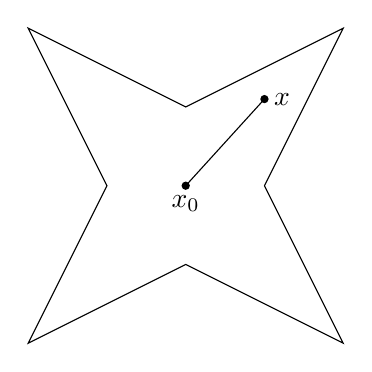
\begin{tikzpicture}
      \draw (1, 0) -- (2, 2) -- (0, 1) -- (-2, 2) -- (-1, 0) -- (-2, -2) -- (0, -1) -- (2, -2) -- (1, 0);
      \node [circ] {};
      \node [below] {$x_0$};
      \draw (0, 0) -- (1, 1.1) node [circ] {} node [right] {$x$};
    \end{tikzpicture}
  \end{center}
  We define $F_t: U \to U$ by
  \[
    F_t(x) = tx + (1 - t) x_0.
  \]
  Then $F$ is a smooth homotopy from the identity map to $F_0$, the constant map to $x_0$. We clearly have $F_1^*$ being the identity map, and $F_0^*$ is the zero map on $H^p_{\dR}(U)$ for all $p \geq 1$. So we have
  \[
    H_{\dR}^p(U) =
    \begin{cases}
      0 & p \geq 1\\
      \R & p = 0
    \end{cases}.
  \]
\end{eg}

\begin{cor}[Poincar\'e lemma]\index{Poincar\'e lemma}
  Let $U \subseteq \R^n$ be open and star-shaped. Suppose $\omega \in \Omega^p(U)$ is such that $\d \omega = 0$. Then there is some $\sigma \in \Omega^{p - 1}(M)$ such that $\omega = \d \sigma$.
\end{cor}

\begin{proof}
  $H^p_{\dR}(U) = 0$ for $p \geq 1$.
\end{proof}

More generally, we have the following notion.

\begin{defi}[Smooth homotopy equivalence]\index{smooth homotopy equivalence}
  We say two manifolds $M, N$ are \emph{smoothly homotopy equivalent} if there are smooth maps $F: M \to N$ and $G: N \to M$ such that both $F \circ G$ and $G \circ F$ are homotopic to the identity.
\end{defi}

\begin{cor}
  If $M$ and $N$ are smoothly homotopy equivalent, then $H_{\dR}^p(M) \cong H_{\dR}^p(N)$.
\end{cor}

Note that by approximation, it can be shown that if $M$ and $N$ are homotopy equivalent as topological spaces (ie. the same definition where we drop the word ``smooth''), then they are in fact smoothly homotopy equivalent. So the de Rham cohomology depends only on the homotopy type of the underlying topological space.

We now want to state the Mayer-Vietoris theorem. This will allow us to compute de Rham cohomology groups by looking at the de Rhaml cohomology of open submanifolds. To do so, we need the language of chain complexes and exact sequences.

\begin{defi}[Cochain complex and exact sequence]\index{cochain complex}\index{exact sequence}
  A sequence
  \[
    \begin{tikzcd}
      \cdots \ar[r] & V_{p - 1} \ar[r, "\d_{p - 1}"] & V_p \ar[r, "\d_p"] & V_{p + 1} \ar[r] & \cdots
    \end{tikzcd}
  \]
  is a \emph{cochain complex} if $\d_p \circ \d_p{p - 1} = 0$ for all $p$.

  It is \emph{exact at $p$} if $\ker \d_p = \im \d_{p - 1}$, and \emph{exact} if it is exact at every $p$.
\end{defi}

\begin{eg}
  The \term{de Rhan complex}
  \[
    \begin{tikzcd}
      \Omega^0(M) \ar[r, "\d"] & \Omega^1(M) \ar[r, "\d"] & \Omega^2(M) \ar[r] & \cdots
    \end{tikzcd}
  \]
  is a cochain complex as $\d^2 = 0$. It is exact at $p$ iff $H_{\dR}^p(M) = \{0\}$.
\end{eg}

\begin{defi}[Cohomology]\index{cohomology}
  Let
  \[
    \begin{tikzcd}
      \cdots \ar[r] & V_{p - 1} \ar[r, "\d_{p - 1}"] & V_p \ar[r, "\d_p"] & V_{p + 1} \ar[r] & \cdots
    \end{tikzcd}
  \]
  be a cochain complex. The \emph{cohomology} is given by
  \[
    H^p(V_{\Cdot}) = \frac{\ker \alpha_p}{\im \alpha_{p - 1}}.
  \]
\end{defi}

\begin{eg}
  The cohomology of the de Rham complex is de Rham cohomology.
\end{eg}

\begin{defi}[Cochain map]\index{cochain map}
  Let $V_{\Cdot}$ and $W_\Cdot$ be cochain complexes. A \emph{cochain map} $V_{\Cdot} \to W_{\Cdot}$ is a map $f_p: V_p \to W_p$ such that the following diagram commutes for all $p$:
   \[
     \begin{tikzcd}
       V_p \ar[r, "f_p"] \ar[d, "\d_p"] & W_n \ar[d, "\d_p"]\\
       V_{p + 1} \ar[r, "f_{p + 1}"] & W_{p + 1}
     \end{tikzcd}
   \]
\end{defi}

\begin{prop}
  A cochain map induces a well-defined homomorphism on the cohomology groups.
\end{prop}

\begin{defi}[Short exact sequence]
  A \term{short exact sequence} is an exact sequence of the form
  \[
    \begin{tikzcd}
      0 \ar[r] & V_1 \ar[r, "\alpha"] & V_2 \ar[r, "\beta"] & V_3 \ar[r] & 0
    \end{tikzcd}.
  \]
  This implies that $\alpha$ is injective, $\beta$ is surjective, and $\im (\alpha) = \ker(\beta)$. By the rank-nullity theorem, we know
  \[
    \dim V_2 = \rank(\beta) + \mathrm{null}(\beta) = \dim V_3 + \dim V_1.
  \]
\end{defi}

\begin{eg}
  If we have an exact sequence such that $\dim V_p < \infty$ for all $p$ and are zero for all but finitely many $p$, then
  \[
    \sum_p (-1)^p \dim V_p = 0.
  \]
\end{eg}

\begin{thm}[Mayer-Vietoris theorem]\index{Mayer-Vietoris sequence}
  Let $M$ be a manifold, and $M = U \cup V$, where $U, V$ are open. We denote the inclusion maps as follows:
  \[
    \begin{tikzcd}
      U \cup V \ar[r, "i_1", hook] \ar[d, "i_2", hook] & U \ar[d, hook, "j_1"]\\
      V \ar[r, hook, "j_2"] & M
    \end{tikzcd}.
  \]
  Then there exists a natural linear map
  \[
    \delta^p_\dR (U \cap V) \to H_{\dR}^{p + 1}(M)
  \]
  such that the following sequence is exact:
  \[
    \begin{tikzcd}
      H^p_{\dR}(M) \ar[r, "j_1^* \oplus j_2^*"] & H^p_{\dR}(U) \oplus H^p_{\dR}(V) \ar[r, "i_1^* - i_2^*"] & H_\dR^p(U \cap V)\ar[out=0, in=180, looseness=2, overlay, lld, "\delta"]\\
      H_\dR^{p+1}(M) \ar[r, "j_1^* \oplus j_2^*"] & H_\dR^{p+1}(U) \oplus H_\dR^{p+1}(V) \ar[r, "i_1^* - i_2^*"] & \cdots
    \end{tikzcd}
  \]
  Here the sequence ends with at $0$ at the left end.
\end{thm}

\begin{eg}
  Consider $M = S^1$. We can cut the circle up :
  \begin{center}
    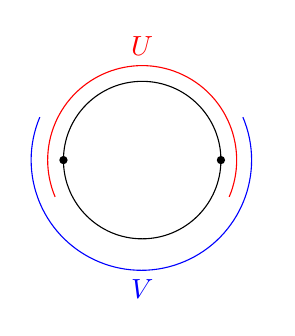
\begin{tikzpicture}
      \draw circle [radius=1];
      \draw [red] (1.105, -0.4673) arc(-22.9:202.9:1.2);
      \node [red, above] at (0, 1.2) {$U$};

      \draw [blue] (1.279, 0.545) arc(22.9:-202.9:1.4);
      \node [blue, below] at (0, -1.4) {$V$};

      \node [circ] at (1, 0) {};
      \node [circ] at (-1, 0) {};
    \end{tikzpicture}
  \end{center}
  Here we have
  \begin{align*}
    S^1 &= \{(x, y): x^2 + y^2 = 1\}\\
    U &= S^1 \cap \{y > -\varepsilon\}\\
    V &= S^1 \cap \{y < \varepsilon\}.
  \end{align*}
  As $U, V$ are diffeomorphic to intervals, hence contractible, and $U \cap V$ is diffeomorphic to the disjoint union of two intervals, we know their de Rham cohomology.
  \[
    \begin{tikzcd}
      0 \ar[r] & H^0_{\dR}(S^1) \ar[r] & H^0_{\dR}(U) \oplus H^0_{\dR}(V) \ar[r] & H_\dR^0(U \cap V)\ar[out=0, in=180, looseness=2, overlay, lld]\\
      & H_\dR^1(S^1) \ar[r] & H_\dR^1(U) \oplus H_\dR^1(V) \ar[r] & \cdots
    \end{tikzcd}
  \]
  We can fill in the things we already know to get
  \[
    \begin{tikzcd}
      0 \ar[r] & \R \ar[r] & \R \oplus \R \ar[r] & \R \oplus \R\ar[out=0, in=180, looseness=2, overlay, lld]\\
      & H_\dR^1(S^1) \ar[r] & 0 \ar[r] & \cdots
    \end{tikzcd}
  \]
  By adding the degrees alternatingly, we know that
  \[
    \dim H^1_{\dR}(S^1) = 1.
  \]
  So
  \[
    H^1_{\dR}(S^1) \cong \R.
  \]
\end{eg}

Now we prove Mayer-Vietoris. The proof splits into two parts --- one differential geometric part, and another algebraic part. The geometric part is the following lemma, and the algebraic part is purely formal, via the snake lemma.

\begin{lemma}
  The following sequence is exact for all $p$:
  \[
    \begin{tikzcd}
      0 \ar[r] & \Omega^p(U \cup V) \ar[r, "j_1^* \oplus j_2^*"] & \Omega^p(U) \oplus \Omega^p(V) \ar[r, "i_1^* - i_2^*"] & \Omega^p(U \cap V) \ar[r] & 0
    \end{tikzcd}
  \]
\end{lemma}
The only non-trivial part is the surjectivity of $i_1^* - i_2^*$. To do so, we need to use the idea of a partition of unity.

\begin{defi}[Partition of unity]\index{partition of unity}
  Let $\{U_\alpha\}$ be an open cover of a manifold $M$. A \emph{partition of unity} subordinate to $\{U_\alpha\}$ is a collection $\varphi_\alpha \in C^\infty(M, \R)$ such that
  \begin{enumerate}
    \item $0 \leq \varphi_\alpha \leq 1$
    \item $\supp(\varphi_\alpha) \subseteq U_\alpha$
    \item For all $p \in M$, all but finitely many $\varphi_\alpha(p)$ are non-zero.
    \item $\sum_\alpha \varphi_\alpha = 1$.
  \end{enumerate}
\end{defi}
This allows us to write any differential form as a sum of forms supported on each $U_\alpha$.

\begin{thm}
  Given any $\{U_\alpha\}$ open cover, there exists a partition of unity subordinate to $\{U_\alpha\}$.
\end{thm}

\begin{proof}
  We will only do the case where $M$ is compact. Given $p \in M$, there exists a coordiante chart $p \in V_p$ and $\alpha(p)$ such that $V_p \subseteq U_{\alpha(p)}$. We pick a bump function $\chi_p \in C^\infty(M, \R)$ such that $\chi_P = 1$ on a neighbourhood $W_p \subseteq V_p$ of $p$. Then $\supp(\chi_p) \subseteq U_{\alpha(p)}$.

  Now by compactness, there are some $p_1, \cdots, p_N$ such that $M$ is covered by $W_{p_1}p \cup \cdots \cup W_{p_N}$. Now let
  \[
    \tilde{\varphi}_\alpha = \sum_{i: \alpha(p_i) = \alpha} \chi_{p_i}.
  \]
  Then by construction, we have
  \[
    \supp(\tilde{\varphi}_\alpha) \subseteq U_\alpha.
  \]
  Also, by construction, we know $\sum_\alpha \tilde{\varphi}_\alpha > 0$. Finally, we let
  \[
    \varphi_\alpha = \frac{\tilde{\varphi}\alpha}{\sum_\beta \tilde{\varphi}_\beta}.
  \]
\end{proof}
The general proof will need the fact that the space is second-countable.

Now we prove our lemma
\begin{proof}[Proof of lemma]
  Let $\{\varphi_U, \varphi_V\}$ be partitions of unity subordinate to $\{U, V\}$. Let $\omega \in \Omega^p(U \cap V)$. We set $\sigma_U \in \Omega^p(U)$ be
  \[
    \sigma_U =
    \begin{cases}
      \varphi_v \omega & \text{on }U \cap V\\
      0 & \text{on }U \setminus \supp \varphi_V
    \end{cases}.
  \]
  Similarly, we define $\sigma_V \in \Omega^p(V)$ by
  \[
    \sigma_V =
    \begin{cases}
      -\varphi_U \omega & \text{on }U \cap V\\
      0 & \text{on }V \setminus \supp \varphi_U
    \end{cases}.
  \]
  Then we have
  \[
    \iota_1^* \sigma_U - \iota_2^* \sigma_V = (\varphi_V \omega + \varphi_U \omega)|_{U \cap V} = \omega.
  \]
  So $\iota_1^* - \iota_2^*$ is surjective.
\end{proof}

We next get to the algebraic part, known as the snake lemma:
\begin{thm}[Snake lemma]\index{snake lemma}
  Suppose we have a short exact sequence of complexes
  \[
    \begin{tikzcd}
      0 \ar[r] & A_{\Cdot} \ar [r, "i"] & B_{\Cdot} \ar [r, "q"] & C_{\Cdot} \ar[r] & 0
    \end{tikzcd},
  \]
  ie. the $i, q$ are chain maps and we have a short exact sequence
  \[
    \begin{tikzcd}
      0 \ar[r] & A_p \ar [r, "i_p"] & B_p \ar [r, "q_p"] & C_p \ar[r] & 0
    \end{tikzcd},
  \]
  for each $p$.

  Then there are maps
  \[
    \delta: H_n(C_{\Cdot}) \to H_{n + 1}(A_{\Cdot})
  \]
  such that there is a long exact sequence
  \[
    \begin{tikzcd}
      \cdots \ar [r] & H_n(A) \ar[r, "i_*"] & H_n(B) \ar[r, "q_*"] & H_n(C) \ar[out=0, in=180, looseness=2, overlay, dll, "\delta"']\\
      & H_{n + 1}(A) \ar[r, "i_*"] & H_{n + 1}(B) \ar[r, "q_*"] & H_{n + 1}(C) \ar [r] & \cdots
    \end{tikzcd}.
  \]
\end{thm}

\begin{proof}
  Omitted (it can be found in the Algebraic topology notes). % maybe do copy and paste.
\end{proof}

\section{Integration}
\subsection{Orientation}
Before we can talk about integration, we need to have the notion of an orientation.

Informally, an orientation on a vector space $V$ is a choice of collection of ordered basis that we declare to be ``oriented''. If $(e_1, \cdots, e_n)$ is an oriented bases, then changing the sign of one of the $e_i$ changes orientation, while scaling by a positive multiple does not.
\begin{defi}[Orientation of vector space]\index{orientation!vector space}
  Let $V$ be a vector space with $\dim V = n$. An \emph{orientation} is an element $\omega \in\Lambda^n (V^*)$, up to equivalence $\omega \sim \omega'$ iff $\omega = \lambda \omega'$. A basis $\{e_1, \cdots, e_n\}$ is \emph{oriented} if
  \[
    \omega(e_1, \cdots, e_n) > 0.
  \]
  By convention, if $V = \{0\}$, an orientation is just a choice of number in $\{\pm\}$.
\end{defi}

Suppose we have picked an oriented basis $e_1, \cdots, e_n$. If we have any other basis $\tilde{e}_1, \cdots, \tilde{e}_n$, we write
\[
  e_i = \sum_j B_{ij} \tilde{e}_j.
\]
Then we have
\[
  \omega (\tilde{e}_1, \cdots, \tilde{e}_n) = \det B \omega(e_1, \cdots, e_n).
\]
So $\tilde{e}_1, \cdots, \tilde{e}_n$ is oriented iff $\det B > 0$.

We now generalize this to manifolds, where we try to orient the tangent bundle smoothly.

\begin{defi}[Orientation of manifold]\index{orientation!manifold}\index{manifold!orientation}
  An \emph{orientation} of a manifold is defined to be an element $\omega \in \Omega^n(M)$ that is nowhere vanishing, up to equivalence given by $ \omega \sim \omega'$ if there is some smooth $f: M \to \R_{> 0}$ such that $\omega = f \omega'$.
\end{defi}

\begin{defi}[Orientable manifold]\index{orientable manifold}\index{manifold!orientable}
  A manifold is \emph{orientable} if it has some orientation.
\end{defi}

If $M$ is a connected, orientable manifold, then it has precisely two possible orientations.

\begin{defi}[Oriented manifold]\index{oriented manifold}
  An \emph{oriented manifold} is a manifold with a choice of orientation.
\end{defi}

\begin{defi}[Oriented coordinates]\index{oriented coordinates}
  Let $M$ be an oriented manifold. We say coordinates $x_1, \cdots, x_n$ on a chart $U$ are \emph{oriented coordinates} if
  \[
    \left.\frac{\partial}{\partial x_1}\right|_p, \cdots, \left.\frac{\partial}{\partial x_n}\right|_p
  \]
  is an oriented basis for $T_p M$ for all $p \in U$.
\end{defi}
Note that we can always find enough oriented coordinates. Given any connected chart, either the chart is oriented, or $-x_1, \cdots, x_n$ is oriented. So any oriented $M$ is covered by oriented charts.

Now by the previous discussion, we know that if $x_1, \cdots, x_n$ and $y_1, \cdots, y_n$ are oriented bases, then the transition maps for the tangent space all have positive determinant.

\begin{eg}
  $\R^n$ is always assumed to have the standard orientation given by $\d x_1 \wedge \cdots \d x_n$.
\end{eg}

\begin{defi}[Orientation-preserving diffeomorphism]\index{orientation!-preserving diffeomorphism}\index{diffeomorphism!orientation preserving}
  Let $M, N$ be oriented manifolds, and $F \in C^\infty(M, N)$ be a diffeomorphism. We say $F$ \emph{preserves orientation} if $\D F|_p: T_p M \to T_{F(p)}N$ takes an oriented basis to an oriented basis.

  Alternatively, this says the pullback of the orientation on $N$ is the orientation on $M$ (up to equivalence).
\end{defi}

\subsection{Integration on \texorpdfstring{$\R^n$}{Rn}}
We are going to start by stating some facts about integration on $\R^n$.

\begin{defi}[Domain of integration]\index{domain of integration}
  Let $D \subseteq \R^n$. We say $D$ is a \emph{domain of integration} if $D$ is bounded and $\partial D$ has measure zero.
\end{defi}

Since $D$ can be an arbitrary subset, we define an $n$-form on $D$ to be some $\omega \in \Omega^n(U)$ for some open $U$ containing $D$.

\begin{defi}[Integration on $R^n$]\index{integration!on $R^n$}
  Let $D$ be a compact domain of integration, and
  \[
    \omega = f\; \d x_1 \wedge \cdots \wedge \d x_n
  \]
  be an $n$-form on $D$. Then we define
  \[
    \int_D \omega = \int_D f(x_1, \cdots, x_n) \;\d x_1 \cdots \d x_n.
  \]
  In general, let $U \subseteq \R^n$ and let $\omega \in \Omega^n(M)$ have compact support. We define
  \[
    \int_U \omega = \int_D \omega
  \]
  for some $D\subseteq U$ containing the support of $\supp \omega$.
\end{defi}
Note that we do not directly say we integrate it on the $\supp \omega$, since $\supp \omega$ need not have a nice boundary.

What happens to integration when we change variables?

\begin{defi}[Smooth function]\index{smooth function}
  Let $D \subseteq \R^n$ and $F: D \to \R^m$. We say $f$ is smooth if it is a restriction of some smooth function $\tilde{f}: U \to \R^m$ where $U \supseteq D$.
\end{defi}

\begin{lemma}
  Let $f: D \to E$ be a smooth map between domains of integration in $\R^n$, and assume that $F|_{\mathring{D}}: \mathring{D} \to \mathring{E}$ is an orientation-preserving diffeomorphism. Then
  \[
    \int_E \omega = \int_D F^* \omega.
  \]
\end{lemma}
This is exactly what we want. To define integration on a manifold, we want to do it locally on charts, and then patch them up together. This tells us it doesn't matter which chart we choose!

\begin{proof}
  Suppose we have coordinates $x_1, \cdots, x_n$ on $D$ and $y_1, \cdots, y_n$ on $E$. Write
  \[
    \omega = f\;\d y_1 \wedge \cdots \wedge \d y_n.
  \]
  Then we have
  \begin{align*}
    \int_E \omega &= \int_E f\;\d y_1, \cdots, \d y_n\\
    &= \int_D (f \circ F)|\det \D F|\;\d x_1, \cdots, x_n\\
    &= \int_D (f \circ F) \det \D f \; \d x_1, \cdots, \d x_n\\
    &= \int_D F^* \omega.
  \end{align*}
  Here we used the fact that $|\det \D F| = \det \D F$ because $F$ is orientation-preserving.
\end{proof}

We can now define integration over manifolds.

\begin{defi}[Integration on manifolds]\index{integration!manifolds}
  Let $M$ be an oriented manifold. Let $\omega \in \Omega^n(M)$. Suppose that $\supp(\omega)$ is a compact subset of some oriented chart $(U, \varphi)$. We set
  \[
    \int_M \omega = \int_{\varphi(U)} (\varphi^{-1})^* \omega.
  \]
  By the previous lemma, this does not depend on the oriented chart $(U, \varphi)$.

  If $\omega \in \Omega^n(M)$ is a general form with compact support, we do the following: cover $K$ by finitely many oriented charts $\{U_\alpha\}_{\alpha = 1, \ldots, m}$. Let $\{\chi_\alpha\}$ be a partition of unity subordinate to $\{U_\alpha\}$. We then set
  \[
    \int_M \omega = \sum_\alpha \int_{U_\alpha} \chi_\alpha \omega.
  \]
\end{defi}

\begin{lemma}
  This is well-defined, ie. it is independent of cover and partition of unity.
\end{lemma}

Note that it is possible to define this for non-smooth forms, or not-everywhere-defined form, or with non-compact support etc, but we will not do it here.

Also, note that this is purely a theoretical definition. It is absolutely useless for computations, and there is no hope you can evaluate that directly. However, it does give a good definition of integration with the expected properties, eg. linearity.

To actually integrate things, we want to cut up our manifolds into \emph{disjoint} pieces, integrate them up in each piece, and add them up together. It would, in general, not be possible to cover the manifold by disjoint open subsets, but we can try to cover it by some domains of integration.

\begin{defi}[Parametrization]\index{parametrization}
  Let $M$ be either an oriented manifold of dimension $n$, or a domain of integration in $\R^n$. By a \emph{parametrization} of $M$ we mean a decomposition
  \[
    M = S_1 \cup \cdots \cup S_n,
  \]
  with smooth maps $F_i: D_i \to S_i$, where $D_i$ is a compact domain of integration, such that
  \begin{enumerate}
    \item $F_i|_{\mathring{D}_i}: \mathring{D}_i \to \mathring{S}_i$ is an orientation-preserving diffeomorphism
    \item $\partial S_i$ has measure zero (if $M$ is a manifold, this means $\varphi(\partial S_i \cap U)$ for all charts $(U, \varphi)$).
    \item For $i \not= j$, $S_i$ intersects $S_j$ only in their common boundary.
  \end{enumerate}
\end{defi}

\begin{thm}
  Given a parametrization of $M$ and an $o\omega \in \Omega^n(M)$ with compact support, we have
  \[
    \int_M \omega = \sum_i \int_{D_i} F_i^* \omega.
  \]
\end{thm}

\begin{proof}
% We know $M$ is covered by oriented charts $(U_\alpha, \varphi_\alpha)$ such that $\varphi$ gives a smooth map $\varphi: \bar{U}_\alpha \to \overline{B_1(0)}$. We can then pick this cover and a partition of unity subordinate to this cover. Then if we define $\int_M \omega$ this way, it suffices to deal with the case where $\supp(\omega)$ lies in a single chart $(U, \varphi)$. Then identifying $\bar{U}$ with $\overline{B_1(0)}$, it suffices to consider the case where $M = \overline{B_1(0)}$. Then the result is obvious.

  By using partitions of unity, we may consider the case where $\omega$ has support in a single chart, and thus we may wlog we are working on $\R^n$, and then the result is obvious.
\end{proof}

There is a problem --- in all our lives, we've been integrating functions, not forms. If we have a function $f: \R \to \R$, then we can take the integral
\[
  \int f\;\d x.
\]
Now of course, we are not actually integrating $f$. We are integrating the differential form $f\;\d x$. Why we seem like we are integrating functions is because we have a background form $\d x$. So if we have a manifold $M$ with a ``background'' $n$-form $\omega \in \Omega^n (M)$, then we can integrate $f \in C^\infty(M, \R)$ by
\[
  \int_M f \omega.
\]
However, a manifold doesn't usually come with such a canonical form. Fortunately, we do when we have a Riemannian metric.
\begin{lemma}
  Let $M$ be an oriented manifold, and $g$ a Riemannian metric on $M$. Then there is a unique $\omega \in \Omega^n(M)$ such that for all $p$, if $e_1, \cdots, e_n$ is an oriented orthonormal basis of $T_pM$, then
  \[
    \omega(e_1, \cdots, e_n) = 1.
  \]
  We call this the \term{Riemannian volume form}, written \term{$\d V_g$}.
\end{lemma}
Note that $\d V_g$ is a notation. It is not the exterior derivative of some mysterious object $V_g$.

\begin{proof}
  Uniqueness is clear, since if $\omega'$ is another, then $\omega_p = \lambda \omega'_p$ for some $\lambda$, and evaluating on an orthonormal basis shows that $\lambda = 1$.

  To see existence, let $\sigma$ be any nowhere vanishing $n$-form giving the orientation of $M$. On a small set $U$, pick a frame $s_1, \cdots, s_n$ for $TM|_U$ and apply the Gram-Schmidt process to obtain an orthonormal frame $e_1, \cdots, e_n$, which we may wlog is oriented. Then we set
  \[
    g = \sigma(e_1, \cdots, e_n),
  \]
  which is non-vanishing because $\sigma$ is nowhere vanishing. Then set
  \[
    \omega = \frac{\sigma}{g}.
  \]
  This proves existence locally, and can be patched together globally by uniqueness.
\end{proof}

\section{Stokes Theorem}
Recall from, say, IA Vector Calculus that Stoke's theorem relates an integral on a manifold to a integral on its boundary. However, our manifolds do not have boundaries! So we can't talk about Stoke's theorem! So we now want to define what it means to be a manifold with boundary.

\begin{defi}[Manifold with boundary]\index{manifold!with boundary}\index{chart!with boundary}\index{atlas!with boundary}
  Let
  \[
    \H^n = \{(x_1, \cdots, x_n): \R^n: x_n \geq 0\}.
  \]
  A \emph{chart-with-boundary} on a set $M$ is a bijection $\varphi: U \to \varphi(U)$ for some $U \subseteq M$ such that $\varphi(U) \subseteq H^n$ is open. Note that this image may or may not hit the boundary of $\H^n$. So a ``normal'' chart is also a chart with boundary.

  An \emph{atlas-with-boundary} on $M$ is a cover by charts-with-boundary $(U_\alpha, \varphi_\alpha)$ such that the transition maps
  \[
    \varphi_\beta \circ \varphi_\alpha^{-1}: \varphi_\alpha(U_\alpha \cap U_\beta) \to \varphi_\beta(U_\alpha \cap U_\beta)
  \]
  is smooth (in the usual sense) for all $\alpha, \beta$.

  A \emph{manifold-with-boundary} us a set $M$ with an (equivalence class of) atlas with boundary whose induced topology is Hausdorff and second-countable.
\end{defi}

Note that a manifold with boundary is not a manifold, but a manifold is a manifold with boundary. We will often be lazy and drop the ``with boundary'' descriptions.

\begin{defi}[Boundary point]\index{boundary point}\index{$\partial M$}
  If $M$ is a manifold with boundary and $p \in M$, then we say $p$ is a boundary point if $\varphi(p) \in \partial \H^n$ for some (hence any) chart-with-boundary $(U, \varphi)$ containing $p$. We let $\partial M$ be the set of boundary points and $\Int(M) = M \setminus \partial M$.
\end{defi}

Note that these are not the topological notions of boundary and interior.

\begin{prop}
  Let $M$ be a manifold with boundary. Then $\Int(M)$ and $\partial M$ are naturally manifolds, with
  \[
    \dim \partial M = \dim \Int M - 1.
  \]
\end{prop}

\begin{eg}
  The solid ball $\overline{B_1(0)}$ is a manifold with boundary, whose interior is $B_1(0)$ and boundary is $S^{n - 1}$.
\end{eg}

Note that the product of manifolds with boundary is not a manifold with boundary. For example, the interval $[0, 1]$ is a manifold with boundary, but $[0, 1]^2$ has \emph{corners}. This is bad. We can develop the theory of manifolds with corners, but that is more subtle. We will not talk about them.

Everything we did for manifolds can be done for manifolds with boundary, eg. smooth functions, tangent spaces, tangent bundles etc. Note in particular the definition of the vector space as derivations still work word-for-word.

\begin{lemma}
  Let $p \in \partial M$, say $p \in U \subseteq M$ where $(U, \varphi)$ is a chart (with boundary). Then
  \[
    \left.\frac{\partial }{\partial x_1}\right|_p, \cdots, \left.\frac{\partial}{\partial x_n}\right|_p
  \]
  is a basis for $T_p M$. In particular, $\dim T_p M = n$.
\end{lemma}

\begin{proof}
  Since this is a local thing, it suffices to prove it for $M = \H^n$. We fix $a \in \partial \H^n$. Then
  \[
    C^\infty(\H, \R) = \{f: \H^n \to \R^: f \text{ extends to a smooth function on an open neighbourhood of }\H^n\}.
  \]
  Then by definition, we have
  \[
    T_aH^n = \Der_a(C^\infty(\H^n, \R)).
  \]
  We let $i_*: T_a\H^n \to T_a \R^n$ be given by
  \[
    \iota_*(X) (g) = X(g|_{\H^n})
  \]
  We claim that $i_*$ is an isomorphism. For injectivity, suppose $i_*(X) = 0$. If $f \in C^\infty(\H^n$, then $f$ extends to a smooth $g$ on some neighbourhood $U$ of $\H^n$. Then
  \[
    X(f) = X(g|_{\H^n}) = i_*(X)(g) = 0.
  \]
  So $X(f) = 0$ for all $f$. Then $X = 0$. So $i_*$ is injective.

  To see surjectivity, let $Y \in T_a \R^n$, and let $X \in T_a\H^n$ be defined by
  \[
    X(f) = Y(g),
  \]
  where $g \in C^\infty(\H^n, \R)$ is any extension of $f$ to $U$. To see this is well-defined, we let
  \[
    Y = \sum \alpha_i \left.\frac{\partial}{\partial x_i}\right|_a..
  \]
  Then
  \[
    Y(g) = \sum_{\alpha_i} \left.\frac{\partial g}{\partial x_i}\right|_a,
  \]
  which only depends on $g|_{\H^n}$, ie. $f$. So $X$ is a well-defined element of $T_a\H^n$, and $i_*(X) = Y$ by construction. So done.
\end{proof}

Now we want to see how orientations behave. We can define them in exactly the same way as manifolds, and everything works. However, something interesting happens. If a manifold with boundary has an orientation, this naturally induces an orientation of the boundary.
\begin{defi}[Outward/Inward pointing]\index{outward pointing}\index{inward pointing}
  Let $p \in \partial M$. We then have an inclusion $T_p \partial M \subseteq T_p M$. If $X_p \in T_p M$, then
  \[
    X_p = \sum_{i = 1}^n a_i \frac{\partial}{\partial x_i},
  \]
  where $a_i \in \R$. We say $X_p$ is \emph{outward pointing} if $a_n < 0$, and \emph{inward pointing} if $a_n > 0$.
\end{defi}

\begin{defi}[Induced orientation]\index{induced orientation}
  Let $M$ be an oriented manifold with boundary. We say a basis $e_1,\cdots, e_{n - 1}$ is an oriented basis for $T_p \partial M$ if $(X_p, e_1, \cdots, e_{n - 1})$ is an oriented basis for $T_p M$, where $X_p$ is any outward pointing element in $T_p M$. This orientation is known as the \emph{induced orientation}.
\end{defi}

It is an exercise to see that these notions are all well-defined and do not depend on the basis.
\begin{eg}
  We have an isomorphism
  \begin{align*}
    \H^n &\cong \R^{n - 1}\\
    (x_1, \cdots, x_{n - 1}, 0) &\mapsto (x_1, \cdots,. x_n).
  \end{align*}
  So
  \[
    \left.-\frac{\partial}{\partial x_n}\right|_{\partial \H^n}
  \]
  is an outward pointing vector. So we know $x_1, \cdots, x_{n - 1}$ is an oriented chart for $\partial H^n$ iff
  \[
    -\frac{\partial}{\partial x_n}, \frac{\partial}{\partial x_1}, \cdots, \frac{\partial}{\partial x_n}
  \]
  is oriented, which is true iff $n$ is even.
\end{eg}

\begin{eg}
  If $n = 1$, say $M = [a, b] \subseteq \R$ with $a < b$, then $\{a, b\}$, then $T_p \partial M = \{0\}$. So an orientation of $\partial M$ is a choice of numbers $\pm 1$ attached to each point. So the convention is that if $M$ is in the standard orientation induced by $M \subseteq \R$, then the orientation is obtained by giving $+1$ to $b$ and $-1$ to $a$.
\end{eg}

Finally, we get to Stokes' theorem.
\begin{thm}[Stokes' theorem]\index{Stokes' theorem}
  Let $M$ be an oriented manifold with boundary of dimension $n$. Then if $\omega \in \Omega^{n - 1}(M)$ has compact support, then
  \[
    \int_M \d \omega = \int_{\partial M}\omega.
  \]
  In particular, if $M$ has no boundary, then
  \[
    \int_M \d \omega = 0
  \]
\end{thm}
Note that this makes sense. $\d \omega$ is an $n$-form on $M$, so we can integrate it. On the right hand side, what we really doing is integrating the restriction of $\omega$ to $\partial M$, ie. the $(n - 1)$-form $i^* \omega$, where $i: \partial M \to M$ is the inclusion, so that $i^* \omega \in \Omega^{n - 1}(\partial M)$.

Note that if $M = [a, b]$, then this is just the usual fundamental theorem of calculus.

The hard part of the proof is keeping track of the signs.
\begin{proof}
  We first do the case where $M = \H^n$. Then we have
  \[
    \omega = \sum_{i = 1}^n \omega_i\;\d x_1 \wedge \cdots \wedge \widehat{\d x_i} \wedge \cdots \wedge \d x_n,
  \]
  where $\omega_i$ is compactly supported, and the hat denotes omission. So we have
  \begin{align*}
    \d \omega &= \sum_i \d \omega_i \wedge \d x_1 \wedge \cdots \wedge \widehat{\d x_i} \wedge \cdots \wedge \d x_n\\
    &= \sum_i \frac{\partial \omega_i}{\partial x_i} \d x_i \wedge \d x_1 \wedge \cdots \wedge \widehat{\d x_i} \wedge \cdots \wedge \d x_n\\
    &= \sum_i (-1)^{i - 1} \frac{\partial \omega_i}{\partial x_i} \d x_1 \wedge \cdots \wedge \d x_i \wedge \cdots \wedge \d x_n
  \end{align*}
  Let's say
  \[
    \supp(\omega) = \{x_j \in [-R, R]: j = 1, \cdots, n - 1; x_n \in [0, R]\} = A.
  \]
  Then suppose $i \not= n$. Then we have
  \begin{align*}
    &\hphantom{=}\int_{\H^n} \frac{\partial \omega_i}{\partial x_i} \d x_1 \wedge \cdots \wedge \d x_i \wedge \cdots \wedge \d x_n\\
    &= \int_A \frac{\partial \omega_i}{\partial x_i} \d x_1 \cdots \d x_n\\
    &= \int_{-R}^R \int_{-R}^R \cdots \int_{-R}^R \int_0^R \frac{\partial\omega_i}{\partial x_i}\;\d x_1 \cdots \d x_n\\
    \intertext{By Fubini's theorem, we can integrate this in any order. We integrate with respect to $\d x_i$ first. So this is}
    &= \pm \int_{-R}^R \cdots \int_{-R}^R \int_0^R \left(\int_{-R}^R \frac{\partial \omega_i}{\partial x_i}\;\d x_i\right)\d x_1 \cdots \widehat{\d x_i} \cdots \d x_n
  \end{align*}
  By the fundamental theorem of calculus, the inner integral is
  \[
    \omega(x_1, \cdots, x_{i - 1}, R, x_{i + 1}, \cdots, x_n) - \omega(x_1, \cdots, x_{i - 1}, -R, x_{i + 1}, \cdots, x_n) = 0 - 0 = 0.
  \]
  So the integral vanishes. So we are only left with the $i = n$ term. So we have
  \begin{align*}
    \int_{\H^n} \d \omega &= (-1)^{n - 1} \int_A \frac{\partial u_n}{\partial x_n} \;\d x_1 \cdots \d x_n\\
    &= (-1)^{n - 1} \int_{-R}^R \cdots \int_{-R}^R \left(\int_0^R \frac{\partial \omega_n}{\partial x_n}\;\d x_n\right) \d x_1 \cdots \d x_{n - 1}
  \end{align*}
  Now that integral is just
  \[
    u_n(x_1, \cdots, x_{n - 1}, R) - u_n(x_1, \cdots, x_n, 0) = -u_n(x_1, \cdots, x_n, 0).
  \]
  So this becomes
  \[
    =(-1)^n \int_{-R}^R \cdots \int_{-R}^R \omega_n(x_1, \cdots, x_{n - 1}, 0)\;\d x_1 \cdots \d x_{n - 1}.
  \]
  Next we see that
  \[
    i^* \omega = \omega_n \d x_1 \wedge \cdots \wedge \d x_{n - 1},
  \]
  as $i^*(\d x_n) = 0$. So we have
  \[
    \int_{\partial \H^n} i^* \omega = \pm \int_{A \cap \partial H^n} \omega(x_1, \cdots, x_{n - 1}, 0) \d x_1 \cdots \d x_n.
  \]
  Here the sign is a plus iff $x_1, \cdots, x_{n - 1}$ are an oriented coordinate for $\partial \H^n$, ie. $n$ is even. So this is
  \[
    \int_{\partial \H^n} \omega = (-1)^n \int_{-R}^R \cdots \int_{-R}^R \omega_n(x_1, \cdots, x_{n - 1}, 0)\;\d x_1, \cdots, \d x_{n - 1} = \int_{\H^n} \d \omega.
  \]
  Now for a general manifold $M$, suppose first that $\omega \in \Omega^{n - 1}(M)$ is compactly supported in a single oriented chart $(U, \varphi)$. Then the result is true by working in local coordinates. More explicitly, we have
  \[
    \int_M \d \omega = \int_{\H^n}(\varphi^{-1})^* \d \omega = \int_{\H^n} \d((\varphi^{-1})^* \omega) = \int_{\partial \H^n} (\varphi^{-1})^* \omega = \int_{\partial M} \omega.
  \]
  Finally, for a general $\omega$, we just cover $M$ by oriented charts $(U, \varphi_\alpha)$, and use a partition of unity $\chi_\alpha$ subordinate to $\{U_\alpha\}$. So we have
  \[
    \omega = \sum \chi_\alpha \omega.
  \]
  Then
  \[
    \d \omega = \sum (\d \chi_\alpha) \omega + \sum \chi_\alpha \d \omega = \d\left(\sum \chi_\alpha\right) \omega + \sum \chi_\alpha \d \omega = \sum \chi_\alpha \d \omega,
  \]
  using the fact that $\sum \chi_\alpha$ is constant, hence its derivative vanishes. So we have
  \[
    \int_M \d \omega = \sum_\alpha \int-M \chi_\alpha \d \omega = \sum_\alpha \int_{\partial M} \chi_\alpha \omega = \int_{\partial M}\omega.
  \]
\end{proof}
Then all the things likes Green's theorem and divergence theorem follow from these.


\printindex
\end{document}
